\documentclass[
  % all of the below options are optional and can be left out
  % course name (default: 2IL50 Data Structures)
  course = {{16-720B Computer Vision}},
  % quartile (default: 3)
  quartile = {{1}},
  % assignment number/name (default: 1)
  assignment = 5\ -\ 3D\ Reconstruction\ \&\ Photometric\ Stereo,
  % student name (default: Some One)
  name = {{Kangle Deng}},
  % student number, NOT S-number (default: 0123456)
  % studentnumber = {{0123456 ; 0314159}},
  % student email (default: s.one@student.tue.nl)
  email = {{kangled@andrew.cmu.edu}},
  % first exercise number (default: 1)
  firstexercise = 1
]{aga-homework}

\usepackage{url}
\usepackage{subfigure}

\begin{document}
\section{Theory: 3D Reconstruction}
\noindent\textbf{Q1.1} Since ${(0,0)^T,(0,0)^T}$ is a pair of point correspondence, we have:

\begin{equation*}
\begin{aligned}
    & (0,0,1) \cdot \left(\begin{array}{ccc}
       F_{11}  &  F_{12} & F_{13} \\
        F_{21} &  F_{22} & F_{23} \\
        F_{31} & F_{32} & F_{33}
    \end{array}
    \right) \cdot \left(
    \begin{array}{c}
         0 \\
         0 \\
         1
    \end{array}
    \right) = 0. \\
    \Rightarrow \qquad & F_{33} = 0.
\end{aligned}

\end{equation*}

\noindent\textbf{Q1.2} Let the translation vector be $t = (t_x, 0, 0)^T$. Since there is no rotation, the essential matrix between 2 cameras is:

\begin{equation*}
    E = [t]_\times = \left(\begin{array}{ccc}
       0  & 0 & 0 \\
       0  & 0 & -t_x \\
       0 & t_x & 0
    \end{array}\right).
\end{equation*}

For any point $\mathbf{x} = (x_0,y_0,1)^T$ in the first camera, it corresponds to an epipolar line in the other camera:
\begin{equation*}
    l' = E\mathbf{x} = (0,-t_x,t_xy_0),
\end{equation*}
which means a line parallel to x-axis.

Similarly, for any point $\mathbf{x'} = (x'_0,y'_0,1)^T$ in the second camera, it corresponds to an epipolar line in the first camera:
\begin{equation*}
    l = E^T\mathbf{x'} = (0,t_x,-t_xy'_0),
\end{equation*}
which also means a line parallel to x-axis.

\noindent\textbf{Q1.3} For any point $\mathbf{x_0} = (x_0,y_0,z_0)$ in World Coordinate System, let $\mathbf{x_1}$ and $\mathbf{x_2}$ be the corresponding points in Camera 1 and 2. So we have:

\begin{equation*}
    \begin{aligned}
        \mathbf{x_1} = R_1 \mathbf{x_0} + t_1, \\
        \mathbf{x_2} = R_2 \mathbf{x_0} + t_2.
    \end{aligned}
\end{equation*}

So,
\begin{equation*}
    \begin{aligned}
      &  \mathbf{x_0} = R_1^T(\mathbf{x_1} - t_1) = R_2^T(\mathbf{x_2} - t_2). \\
      \Rightarrow \qquad & \mathbf{x_2} = R_2R_1^T(\mathbf{x_1} - t_1) + t_2 = R_2R_1^T\mathbf{x_1} - R_2R_1^Tt_1 + t_2.
    \end{aligned}
\end{equation*}

Therefore, $R_{rel} = R_2R_1^T, t_{rel} = - R_2R_1^Tt_1 + t_2$.

For $E$ and $F$, we have:

\begin{equation*}
    \begin{aligned}
      E & = [t_{rel}]_\times R_{rel}, \\
      F & = K^{-T}[t_{rel}]_\times R_{rel}K^{-1}.
    \end{aligned}
\end{equation*}

\noindent \textbf{Q1.4} As shown in Fig. \ref{fig:cv_hw5_q14}, for any point $A$ in 3D world, let $A'$ be its reflection in a plane mirror. Let $O$ be the camera center. Let $x$ and $x'$ be their homogeneous coordinates in Camera Coordinate System. Let $n$ be the normal vector of the mirror plane. 

\begin{figure}
    \centering
    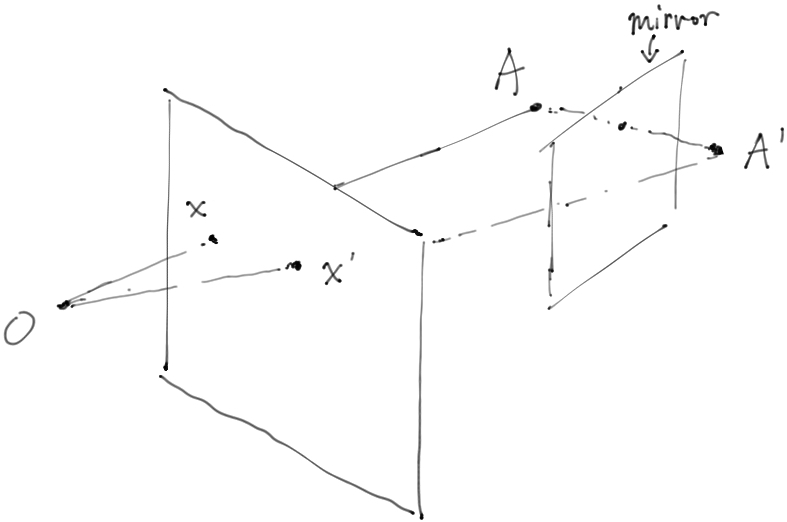
\includegraphics[width=.4\textwidth]{CV/fig/hw5/hw5_14.jpeg}
    \caption{Q1.4}
    \label{fig:cv_hw5_q14}
\end{figure}

Since $AA'$ is perpendicular to the mirror plane, any vector that is perpendicular to plane $OAA'$ is parallel to the mirror plane, and thus perpendicular to $n$. Therefore,

\begin{equation*}
    n^T \cdot (x \times x') = 0.
\end{equation*}

We have the identity equation that:

\begin{equation*}
    x^T \cdot (n \times x') = n^T \cdot (x \times x') = 0.
\end{equation*}
which is equivalent to:

\begin{equation*}
    x^T[n]_\times x' = 0.
\end{equation*}

Since $x$ is arbitrary, the essential matrix is:

\begin{equation*}
    E = [n]_\times.
\end{equation*}
So the fundamental matrix is:

\begin{equation*}
    F = K^{-T}[n]_\times K^{-1}.
\end{equation*}

Note that
\begin{equation*}
    F^T = K^{-T}[n]_\times^T K^{-1} = -K^{-T}[n]_\times K^{-1} = -F.
\end{equation*}

Therefore, $F$ is a skew-symmetric matrix.

\section{Theory: Photometric Stereo}

\noindent\textbf{Q2.1} In Fig.3 (handout), $\Vec{n}$ is the normal vector of the surface, $\Vec{l}$ is the direction of source light, and $\Vec{v}$ is the viewing vector. Lambert's cosine law says:

\begin{equation*}
    L = \frac{\rho_d}{\pi}I\cos\theta = \frac{\rho_d}{\pi} I \cdot \Vec{n} \cdot \Vec{l}.
\end{equation*}

The dot product between $\Vec{l}$ and $\Vec{n}$ comes from $\cos\theta$, where $\theta$ is the angle between $\Vec{l}$ and $\Vec{n}$. This is because we measure the light by the number of photons hitting on the surface per unit area. However, the contact surface gets larger as $\frac{dA}{\cos\theta}$ when $\theta$ is not 0. So the light intensity reaching on the surface is scaled by $\cos\theta$.

Lambert's cosine law describes the diffuse reflection. The object surface is rough enough so that light reflects to each direction equally. Therefore, the viewing direction does not matter.

\noindent\textbf{Q2.2} The tangent plane of $z=f(x,y)$ at $(x,y)$ is spanned by $\{(1,0,f_x)^T, (0,1,f_y)^T\}$. $\mathbf{n}$ is the normal vector of this tangent plane. Therefore,

\begin{equation*}
    \mathbf{n} = k (1,0,f_x)^T \times (0,1,f_y)^T.
\end{equation*}

So,

\begin{equation*}
    \begin{aligned}
      n_1 & = -kf_x, \\
      n_2 & = -kf_y, \\
      n_3 & = k.
    \end{aligned}
\end{equation*}

To remove scale of $\mathbf{n}$, we use the proportion of the elements in $\mathbf{n}$ to denote $f_x$ and $f_y$. Therefore, $f_x = -n_1/n_3, f_y=-n_2/n_3$.

\noindent\textbf{Q2.3} 

\begin{equation*}
\begin{aligned}
      g_x & = \left(\begin{array}{ccc}
       1  & 1 & 1 \\
        1 & 2 & 0 \\
        1 & 1 & 1 \\
        1 & 1 & 1
    \end{array}
    \right), \\
    g_y & = \left(\begin{array}{cccc}
       4  & 4 & 5 & 4 \\
        4 & 4 & 3 & 4 \\
        4 & 4 & 4 & 4
    \end{array}\right).
\end{aligned}

\end{equation*}

Given that $g(0,0) = 1$,

\noindent\textbf{(a)} Use $g_x$ to construct the first row $g(:,0) = [1,2,3,4]$. Then use $g_y$ to construct the rest of $g$:
\begin{equation*}
    \begin{aligned}
          g(:,1) & = [5,6,8,8], \\
          g(:,2) & = [9,10,11,12], \\
          g(:,3) & = [13,14,15,16].
    \end{aligned}
\end{equation*}

So,
\begin{equation*}
    g = \left(\begin{array}{cccc}
        1 & 2 & 3 & 4 \\
        5 & 6 & 8 & 8 \\
        9 & 10 & 11 & 12 \\
        13 & 14 & 15 & 16
    \end{array}\right).
\end{equation*}

\noindent\textbf{(b)} Use $g_y$ to construct the first column $g(0,:)=[1,5,9,13]^T$. Then use $g_x$ to construct the rest of $g$:

\begin{equation*}
    \begin{aligned}
          g(1,:) &= [2,6,10,14]^T, \\
          g(2,:) &= [3,8,11,15]^T, \\
          g(3,:) &= [4,8,12,16]^T. \\
    \end{aligned}
\end{equation*}

So,
\begin{equation*}
    g = \left(\begin{array}{cccc}
        1 & 2 & 3 & 4 \\
        5 & 6 & 8 & 8 \\
        9 & 10 & 11 & 12 \\
        13 & 14 & 15 & 16
    \end{array}\right).
\end{equation*}

These 2 matrices by 2 procedures are the same. It is easy to make $g_x$ and $g_y$ non-integrable. For example, modify $g_x(1,1) = 1$. Then the matrix constructed by procedure (b) changes to:
\begin{equation*}
    \left(\begin{array}{cccc}
        1 & 2 & 3 & 4 \\
        5 & 6 & 7 & 7 \\
        9 & 10 & 11 & 12 \\
        13 & 14 & 15 & 16
    \end{array}\right).
\end{equation*}
while the matrix constructed by procedure (a) does not change. 

We can check whether they're integrable by checking whether $g_{xy} = g_{yx}$. The reason causing the estimated gradients to be non-integrable might be rounding error

\noindent\textbf{Q2.4} 
First perform SVD decomposition of $I$:

\begin{equation*}
    I = U\Sigma V^T.
\end{equation*}

Then select top 3 singular values from $\Sigma$ to form the matrix $\hat{\Sigma}$, whose size is $3\times3$. Then select the corresponding 3 rows from $U$ to form the matrix $\hat{U}$, whose size is $N \times 3$. Also select the corresponding 3 rows from $V$ to form the matrix $\hat{V}$, whose size is $P \times 3$. Since $B$ is the pseudo-normal, set $\hat{B} = \hat{V}^T$. Each column in $\hat{B}$ is a unit normal vector. Then set $\hat{L}^T=\hat{U}\hat{\Sigma}$, so $\hat{L} = \hat{\Sigma}\hat{U}^T$. In this way, $\hat{I} = \hat{L}^T\hat{B} = \hat{U}\hat{\Sigma}\hat{V}^T$ has rank 3.

\section{Practice: 3D Reconstruction}

\subsection{Overview}

\subsection{Fundamental matrix estimation}
\noindent\textbf{Q3.2.1} Fig. \ref{fig:cv_hw5_q321} is the result. The recovered $\mathbf{F}$ is:
\begin{verbatim}
[[ 9.78833286e-10 -1.32135929e-07  1.12585666e-03]
 [-5.73843315e-08  2.96800276e-09 -1.17611996e-05]
 [-1.08269003e-03  3.04846703e-05 -4.47032655e-03]]
\end{verbatim}

\begin{figure}
    \centering
    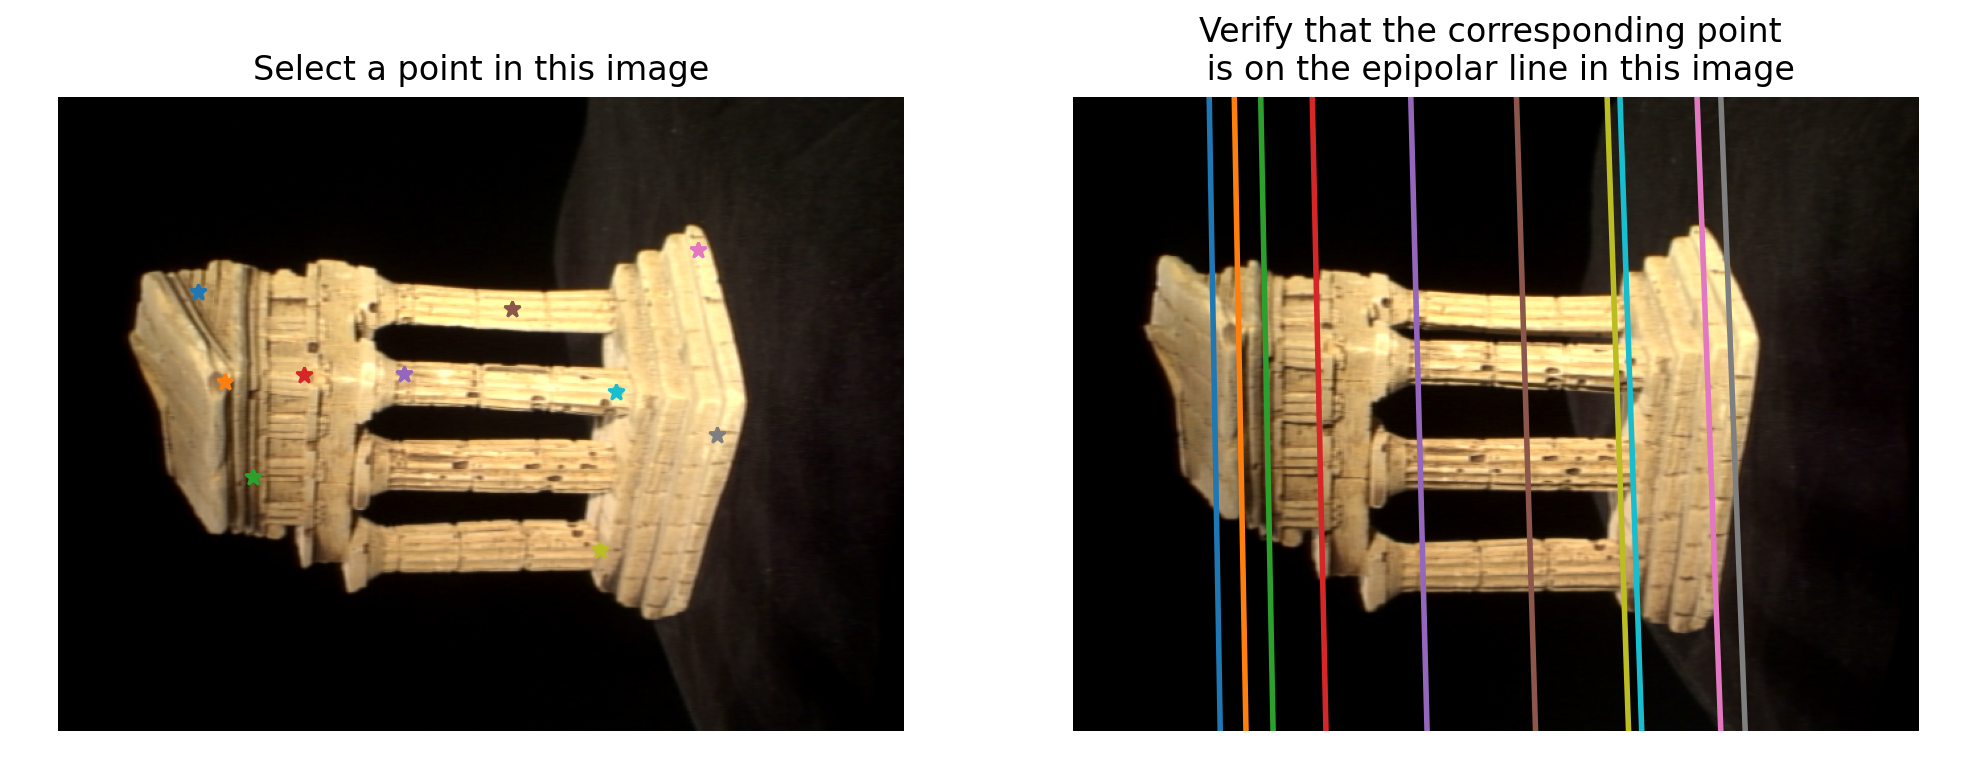
\includegraphics[width=.9\textwidth]{CV/fig/hw5/q321.png}
    \caption{Q3.2.1: Eight-Point Algorithm:  display Epipolar F}
    \label{fig:cv_hw5_q321}
\end{figure}

\noindent\textbf{Q3.2.2}
Fig. \ref{fig:cv_hw5_q322} is the result. The recovered $\mathbf{F}$ is:
\begin{verbatim}
[[ 2.97008877e-09,  3.68954092e-07,  7.28096698e-04],
 [-4.78198323e-07, -2.75453819e-08,  1.60070564e-04],
 [-7.18550554e-04, -1.59779323e-04,  6.46789076e-03]]
\end{verbatim}

\begin{figure}
    \centering
    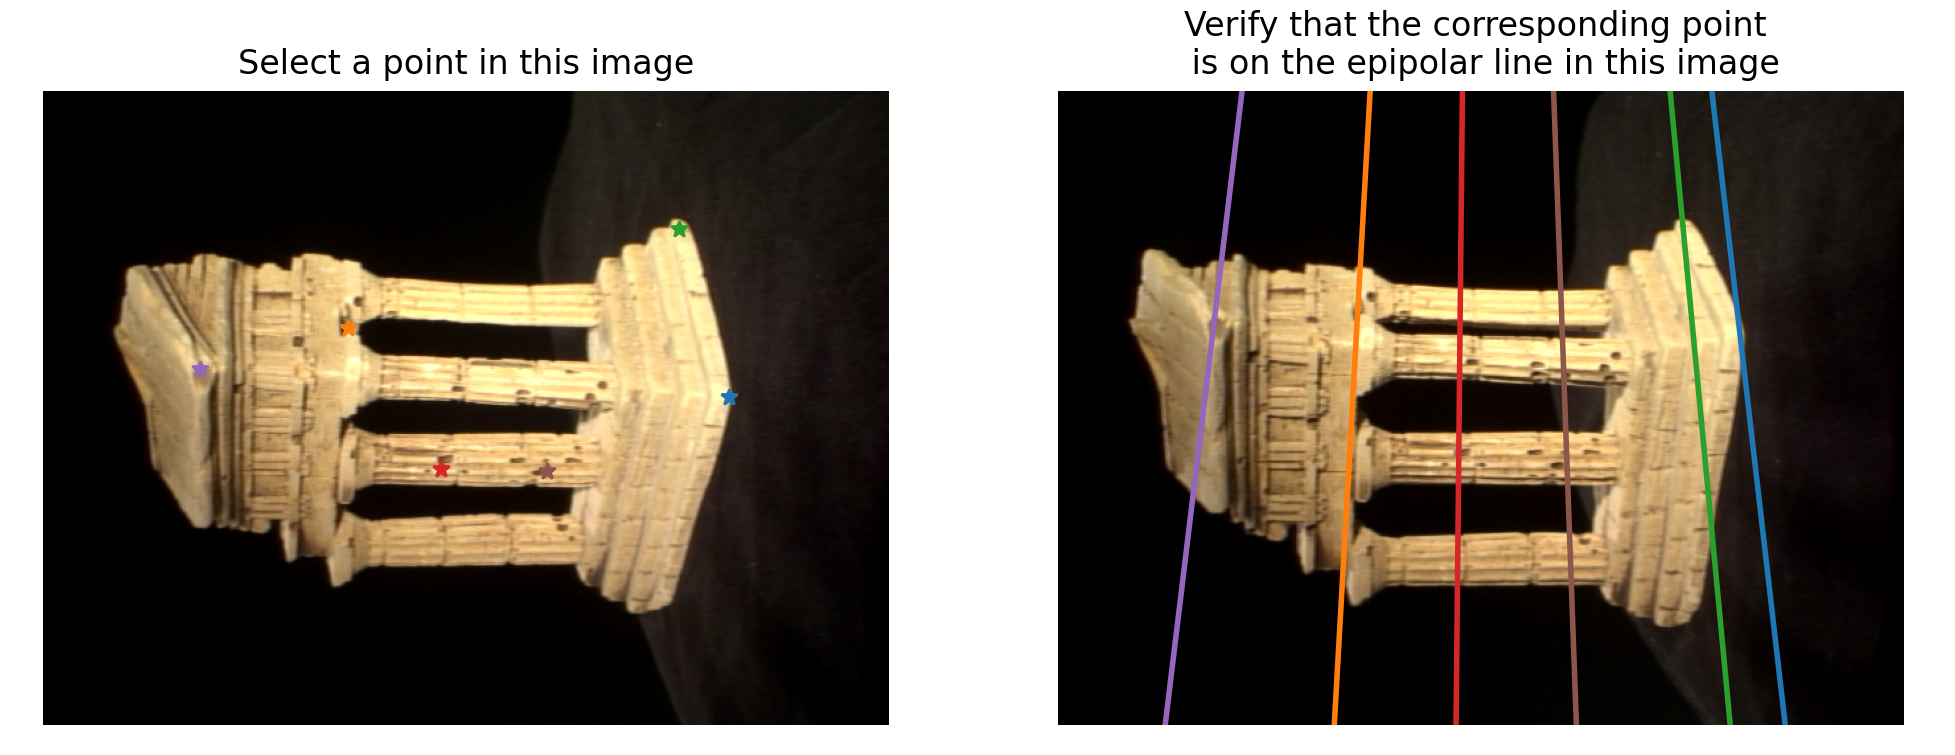
\includegraphics[width=.9\textwidth]{CV/fig/hw5/q3_2_2.png}
    \caption{Q3.2.2: Seven-Point Algorithm:  display Epipolar F}
    \label{fig:cv_hw5_q322}
\end{figure}

\subsection{Metric Reconstruction}
\noindent\textbf{Q3.3.1} The estimated $\mathbf{E}$ is:
\begin{verbatim}
[[ 2.26268684e-03 -3.06552495e-01  1.66260633e+00]
 [-1.33130407e-01  6.91061098e-03 -4.33003420e-02]
 [-1.66721070e+00 -1.33210351e-02 -6.72186431e-04]]
\end{verbatim}

\noindent\textbf{Q3.3.2} Let
\begin{equation*}
    \mathbf{C_1} = \left(\begin{array}{c}
         c_{11}^T \\
         c_{12}^T \\
         c_{13}^T
    \end{array}\right), \qquad \mathbf{C_2} = \left(\begin{array}{c}
         c_{21}^T \\
         c_{22}^T \\
         c_{23}^T
    \end{array}\right).
\end{equation*}

Then
\begin{equation*}
    \begin{aligned}
          \left(\begin{array}{c}
         c_{11}^T \\
         c_{12}^T \\
         c_{13}^T
    \end{array}\right) \cdot \mathbf{w_i} & = \left(\begin{array}{c}
         c_{11}^T\mathbf{w_i} \\
         c_{12}^T\mathbf{w_i} \\
         c_{13}^T\mathbf{w_i}
    \end{array}\right), \\
        \left(\begin{array}{c}
         c_{21}^T \\
         c_{22}^T \\
         c_{23}^T
    \end{array}\right) \cdot \mathbf{w_i} & = 
    \left(\begin{array}{c}
         c_{21}^T\mathbf{w_i} \\
         c_{22}^T\mathbf{w_i} \\
         c_{23}^T\mathbf{w_i}
    \end{array}\right).
    \end{aligned}

\end{equation*}

So
\begin{equation*}
    \begin{aligned}
          \frac{c_{11}^T\mathbf{w_i}}{c_{13}^T\mathbf{w_i}} & = x_{1i}, \\
          \frac{c_{12}^T\mathbf{w_i}}{c_{13}^T\mathbf{w_i}} & = y_{1i}, \\
          \frac{c_{21}^T\mathbf{w_i}}{c_{23}^T\mathbf{w_i}} & = x_{2i}, \\
          \frac{c_{22}^T\mathbf{w_i}}{c_{23}^T\mathbf{w_i}} & = y_{2i}, 
    \end{aligned}
\end{equation*}

Therefore,
\begin{equation*}
    \left(\begin{array}{c}
         c_{11}^T - x_{1i} c_{13}^T  \\
         c_{12}^T - y_{1i} c_{13}^T  \\
         c_{21}^T - x_{2i} c_{23}^T  \\
         c_{22}^T - y_{2i} c_{23}^T  
    \end{array}
    \right) \cdot \mathbf{w_i} = 0.
\end{equation*}

Namely,
\begin{equation*}
    \mathbf{A_i} = \left(\begin{array}{c}
         c_{11}^T - x_{1i} c_{13}^T  \\
         c_{12}^T - y_{1i} c_{13}^T  \\
         c_{21}^T - x_{2i} c_{23}^T  \\
         c_{22}^T - y_{2i} c_{23}^T  
    \end{array}
    \right).
\end{equation*}

\noindent\textbf{Q3.3.3} See the code for implementation.

\subsection{3D Visualization}
\noindent\textbf{Q3.4.1} I use a Gaussian weight window and set the window size as 9. Fig. \ref{fig:cv_hw5_q341} is the result.

\begin{figure}
    \centering
    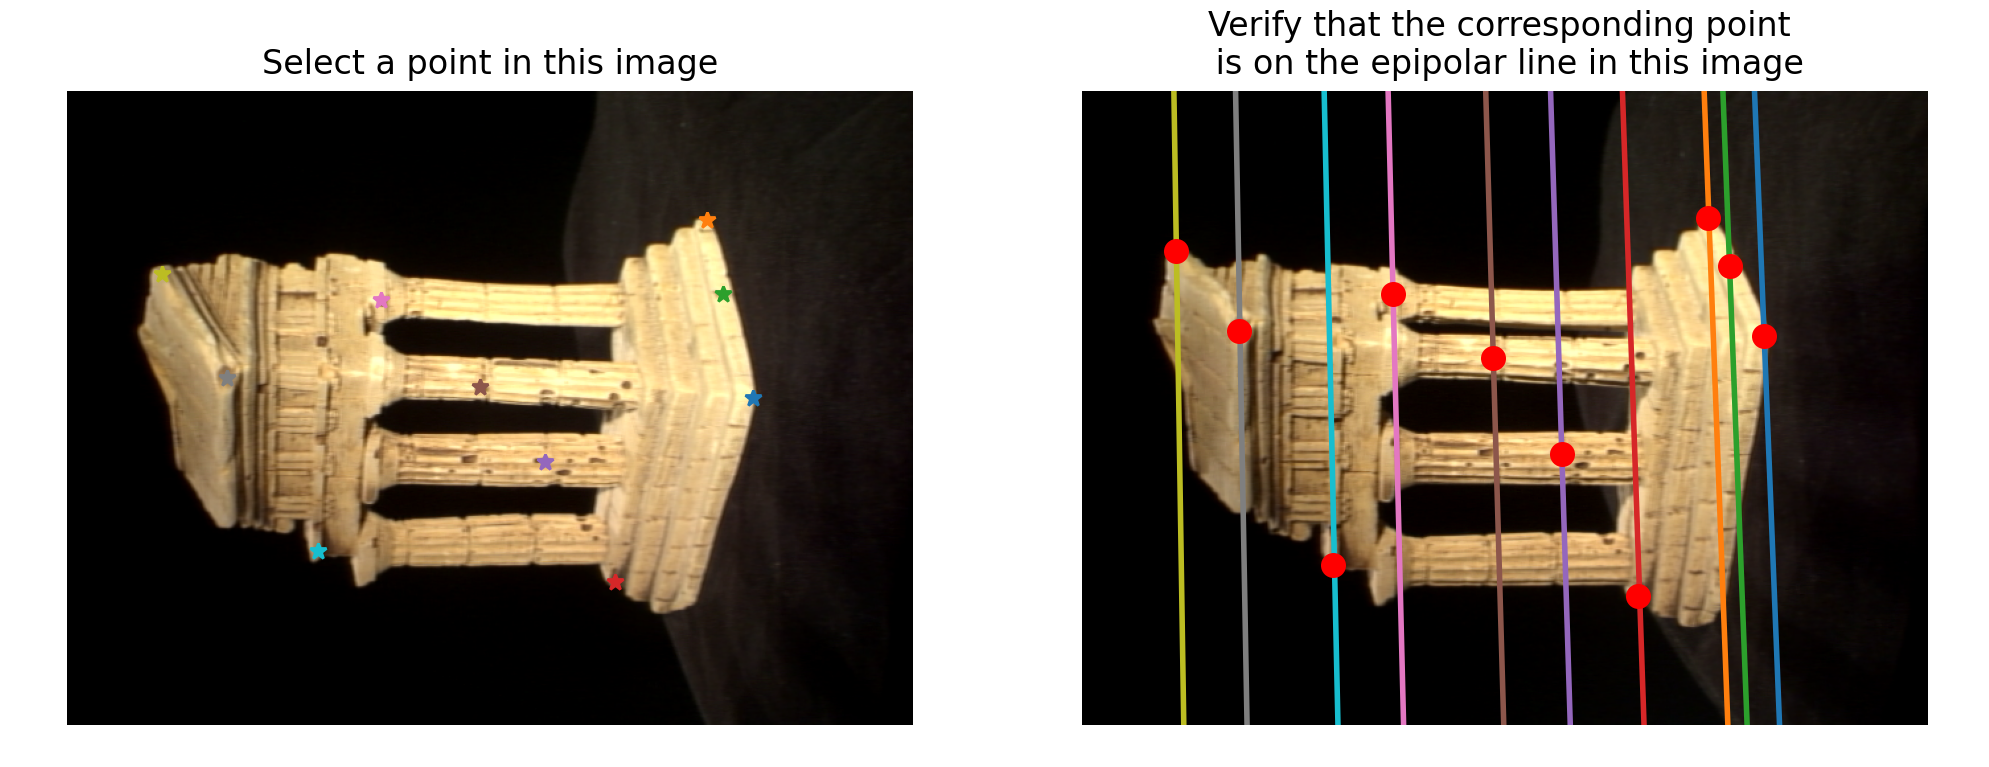
\includegraphics[width=.9\textwidth]{CV/fig/hw5/q341.png}
    \caption{Q3.4.1: detected correspondences}
    \label{fig:cv_hw5_q341}
\end{figure}

\noindent\textbf{Q3.4.2} Fig. \ref{fig:cv_hw5_q342} is the result.

\begin{figure}
    \centering
    \subfigure{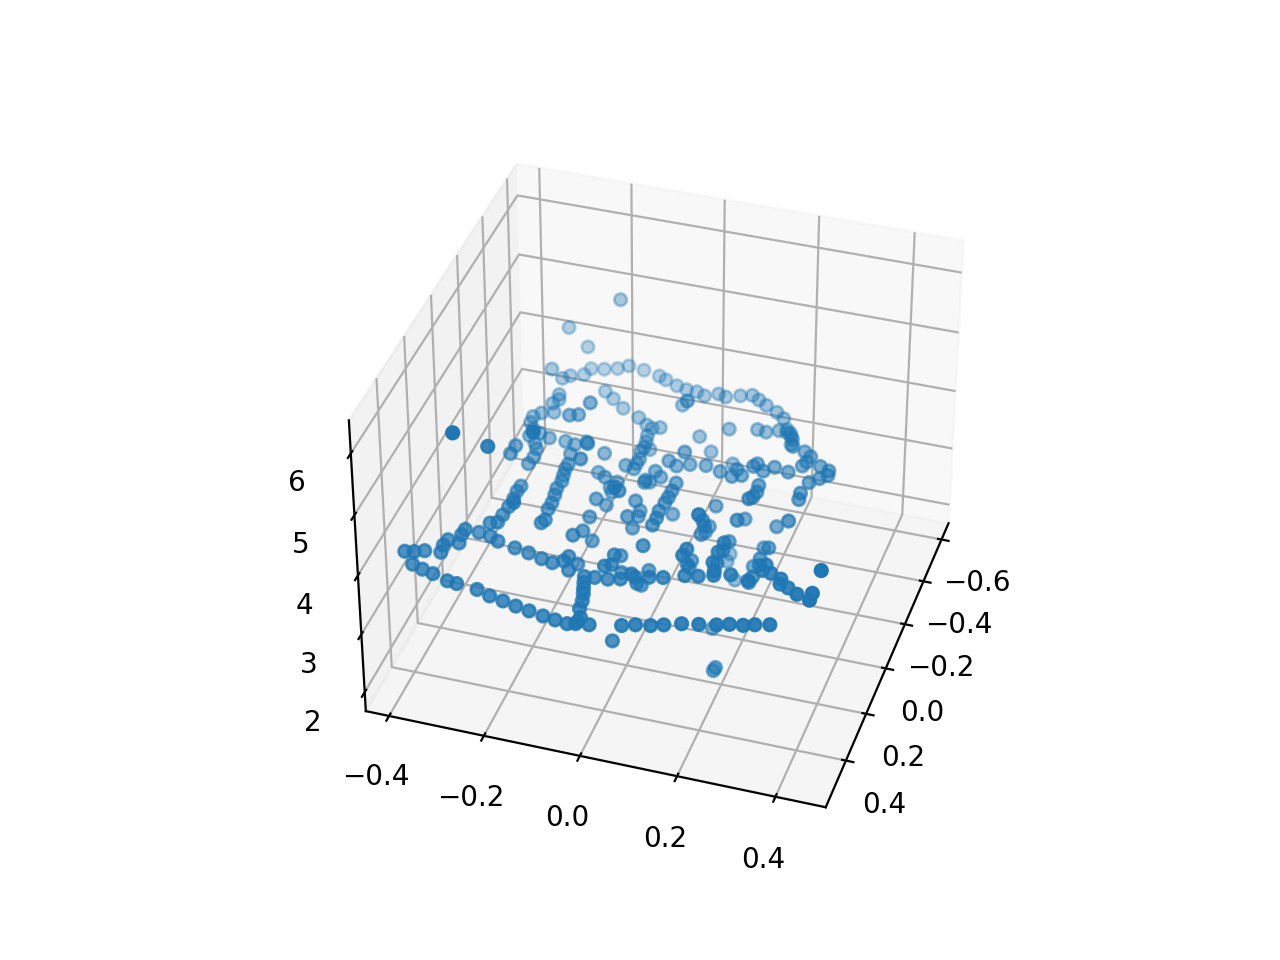
\includegraphics[width=.45\textwidth]{CV/fig/hw5/q342_1.png}}
    \subfigure{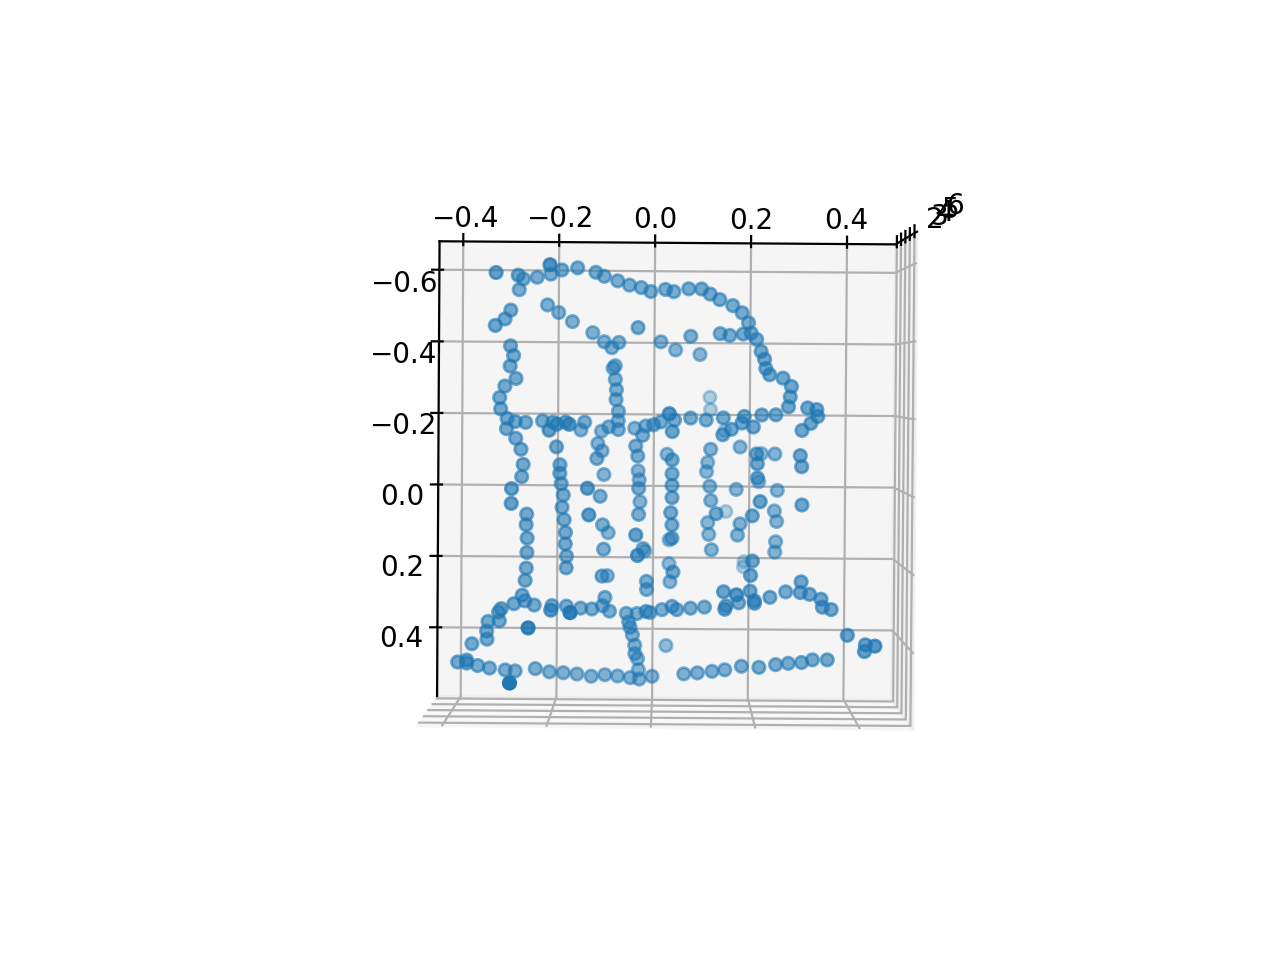
\includegraphics[width=.45\textwidth]{CV/fig/hw5/q342_2.png}}
    \subfigure{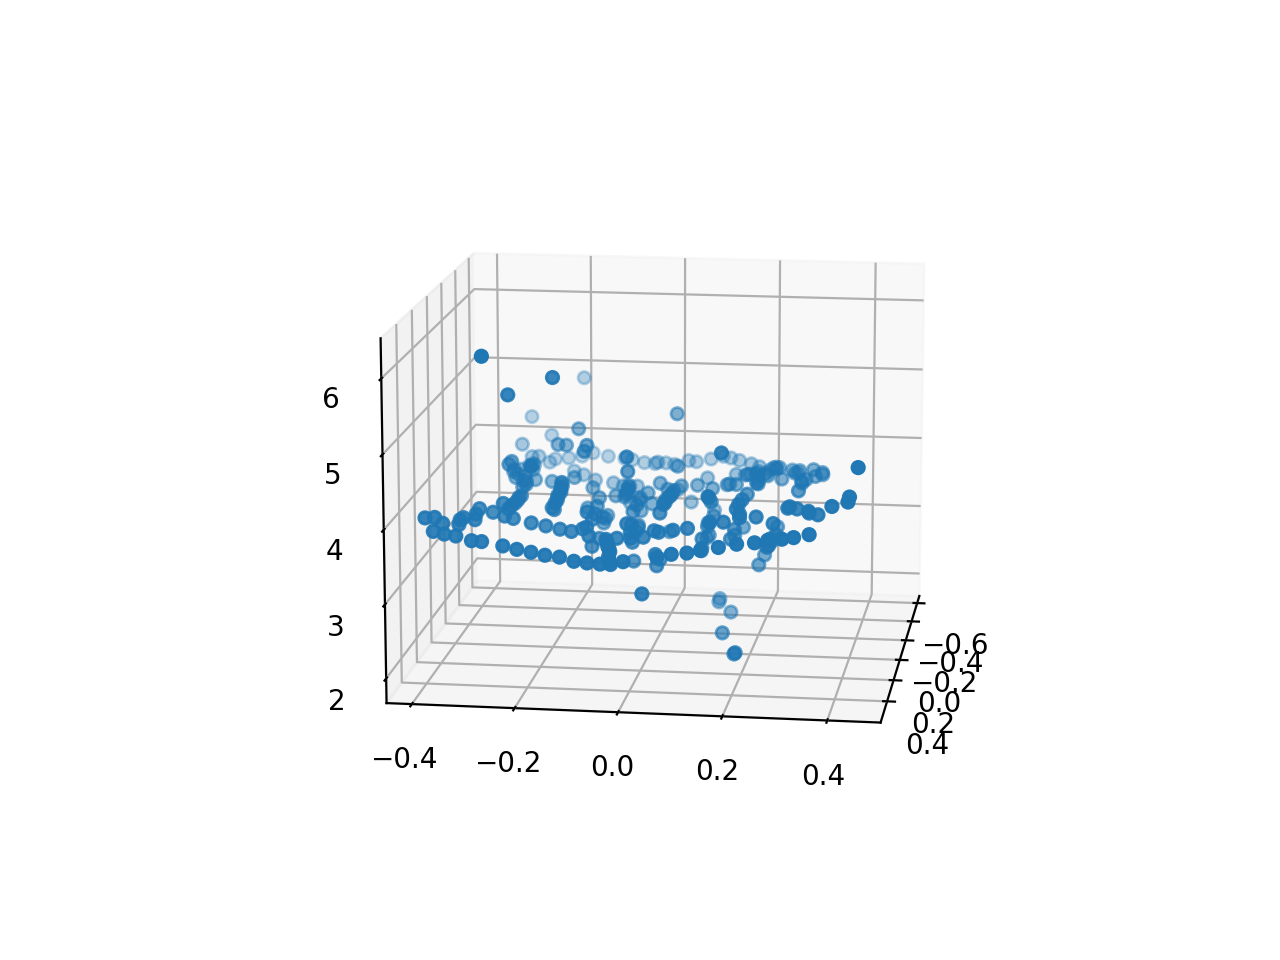
\includegraphics[width=.45\textwidth]{CV/fig/hw5/q342_3.png}}
    \subfigure{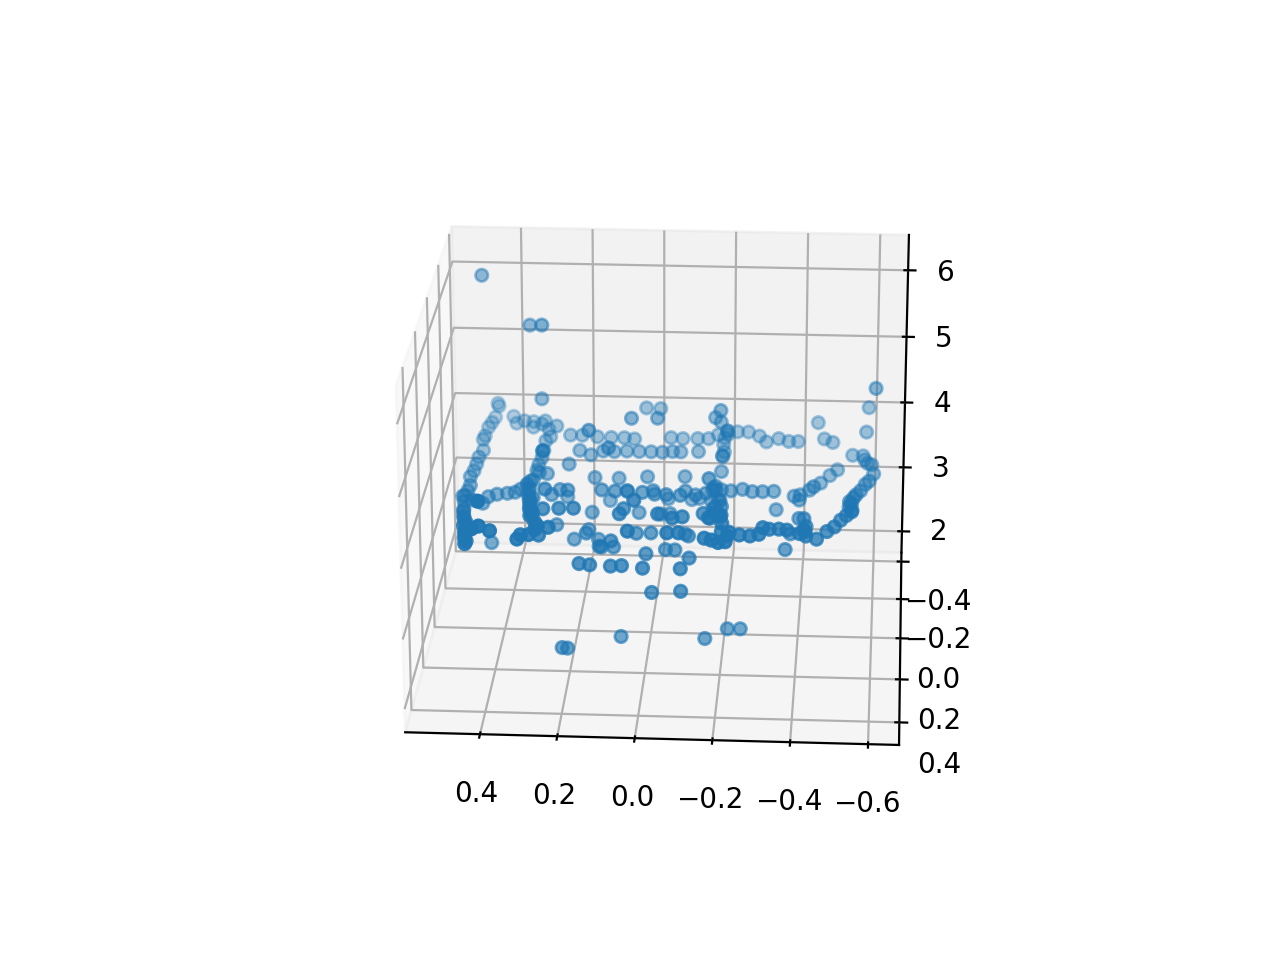
\includegraphics[width=.45\textwidth]{CV/fig/hw5/q342_4.png}}
    \caption{Q3.4.2: Point cloud}
    \label{fig:cv_hw5_q342}
\end{figure}

\subsection{Bundle Adjustment}
\noindent\textbf{Q3.5.1} I use the distance from the point to the epipolar line as the error metric. Note that we can calculate this in either way (from image1 to image2 and vice versa). If the sum of the two-way distances is less than 2, I regard this point as inlier. I iterate the RANSAC for 200 times, and finally get 98 inliers. Fig.\ref{fig:cv_hw5_q351} is the visual result. The fundamental matrix $F$ obtained by RANSAC is:

\begin{verbatim}
[[-5.09523046e-08  5.26246895e-08 -1.19524404e-03]
 [ 1.35061554e-07 -4.86933471e-09  1.95809937e-05]
 [ 1.18142954e-03 -3.52876965e-05  4.03175402e-04]]
\end{verbatim}.

On the other hand, the fundamental matrix $F$ obtained by the eight point algorithm is:

\begin{verbatim}
[[ 2.36832939e-07 -1.50148144e-06  2.45250873e-04]
 [ 1.66554842e-06 -5.26414563e-07 -3.52208862e-04]
 [-4.04922548e-04  5.48651981e-04 -1.45751671e-03]]
\end{verbatim}

\begin{figure}
    \centering
    \subfigure[RANSAC]{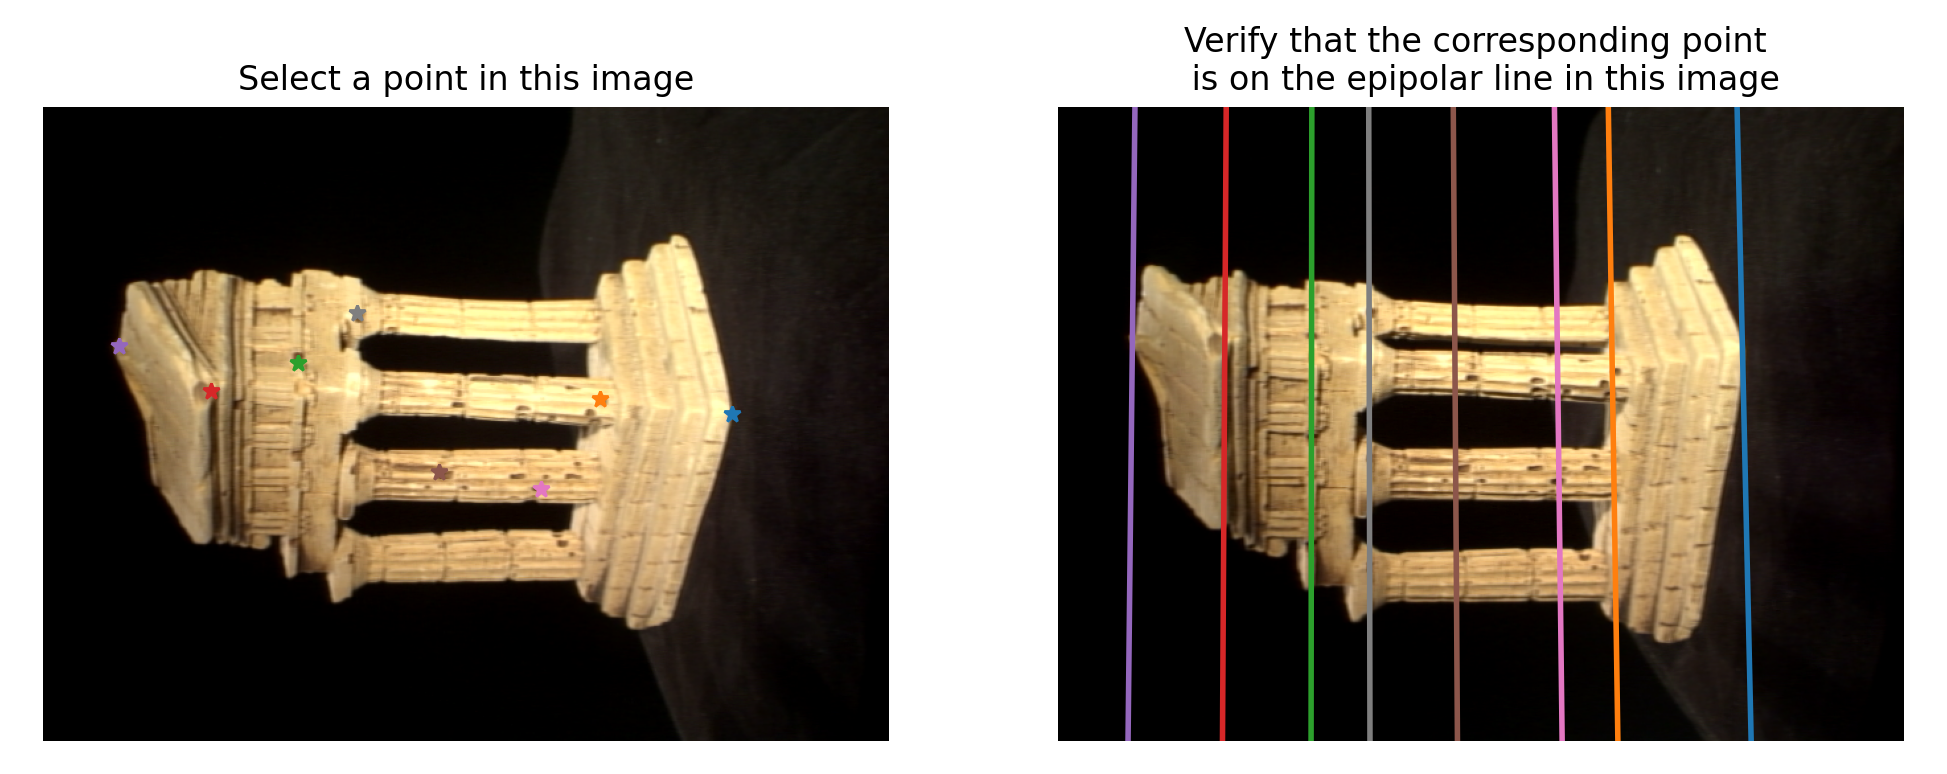
\includegraphics[width=.9\textwidth]{CV/fig/hw5/q351_ransac.png}}
    \subfigure[Eight Point]{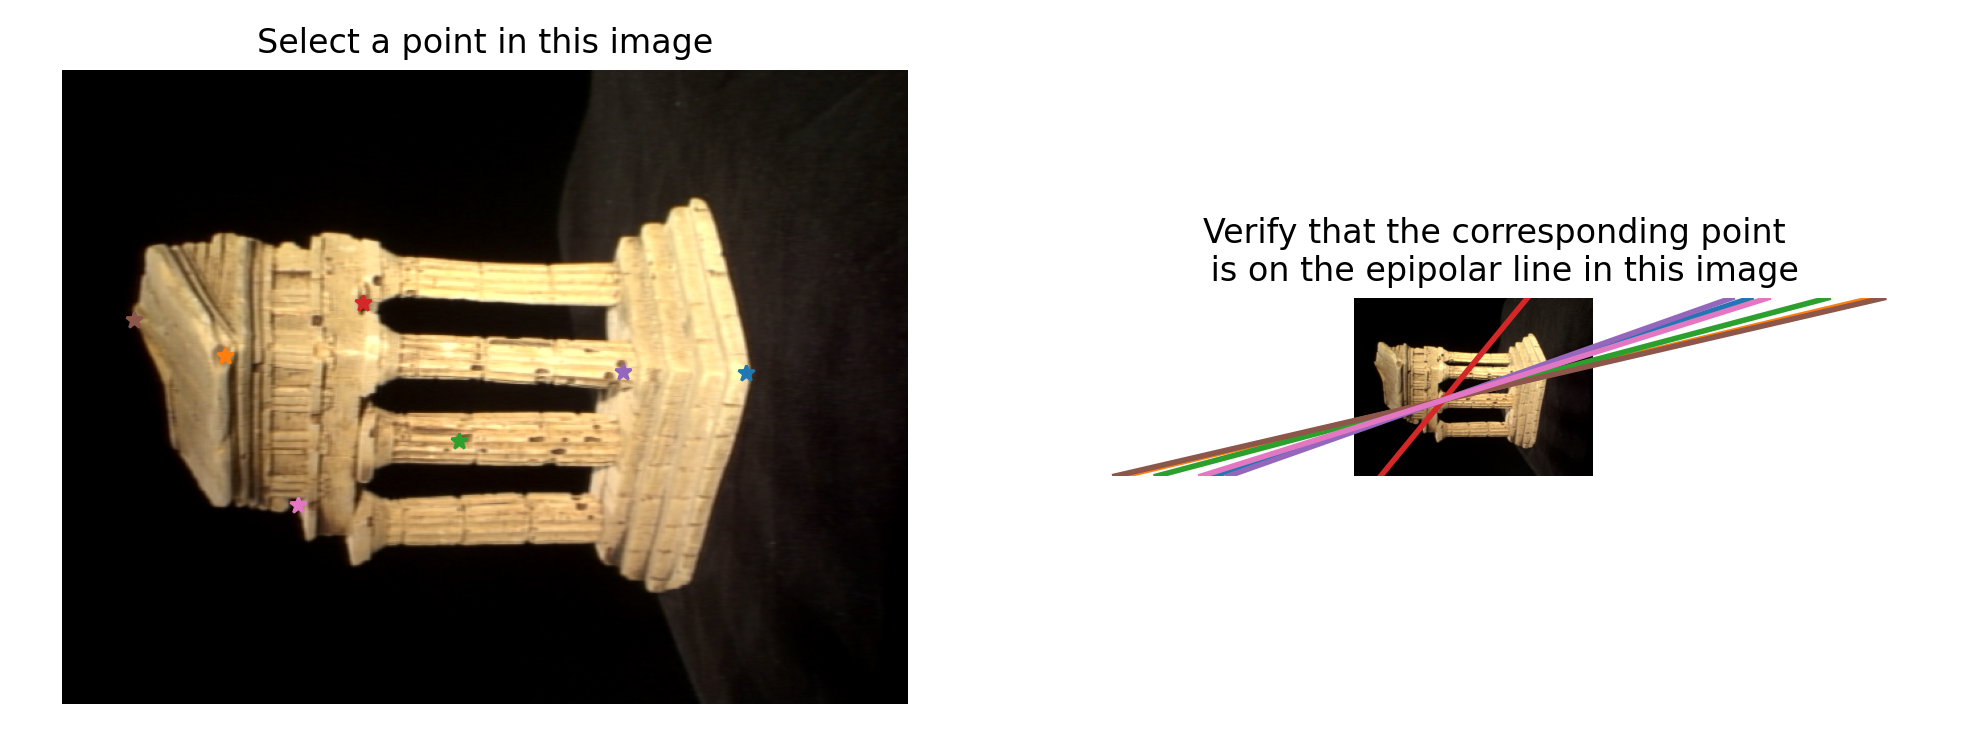
\includegraphics[width=.9\textwidth]{CV/fig/hw5/q351_eightpoint.png}}
    \caption{Q3.5.1: Comparison between RANSAC and Eight-point}
    \label{fig:cv_hw5_q351}
\end{figure}

\noindent\textbf{Q3.5.2} See the code for implementation.

\noindent\textbf{Q3.5.3} Fig. \ref{fig:cv_hw5_q353} is the result. The total reprojection error with initial estimates is $26445.72$ for a total of $104$ inliers, and the optimized reprojection error is $20.85$.

\begin{figure}
    \centering
    \subfigure{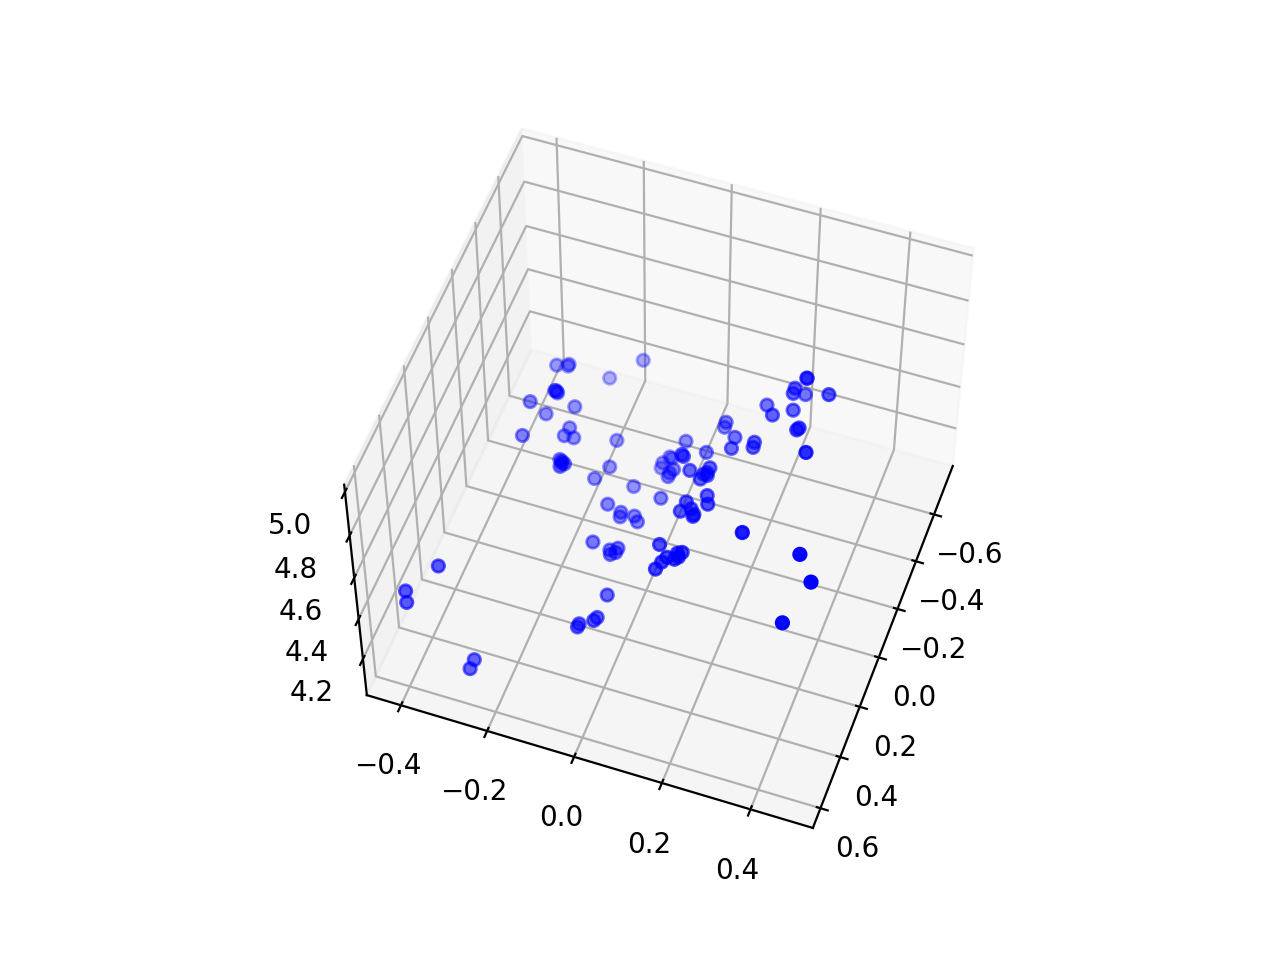
\includegraphics[width=.32\textwidth]{CV/fig/hw5/q353_1_original.png}}
    \subfigure{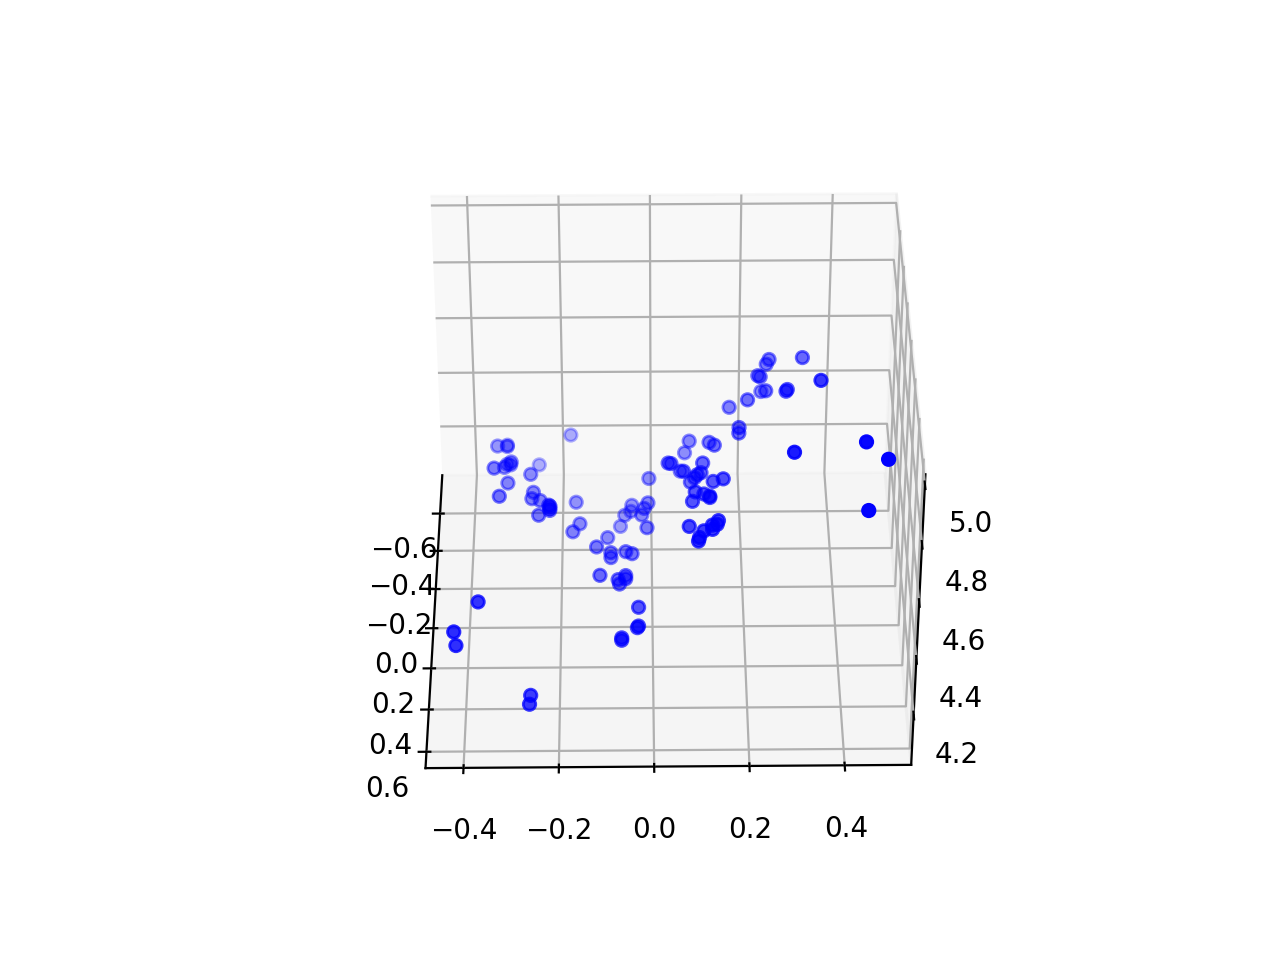
\includegraphics[width=.32\textwidth]{CV/fig/hw5/q353_2_original.png}}
    \subfigure{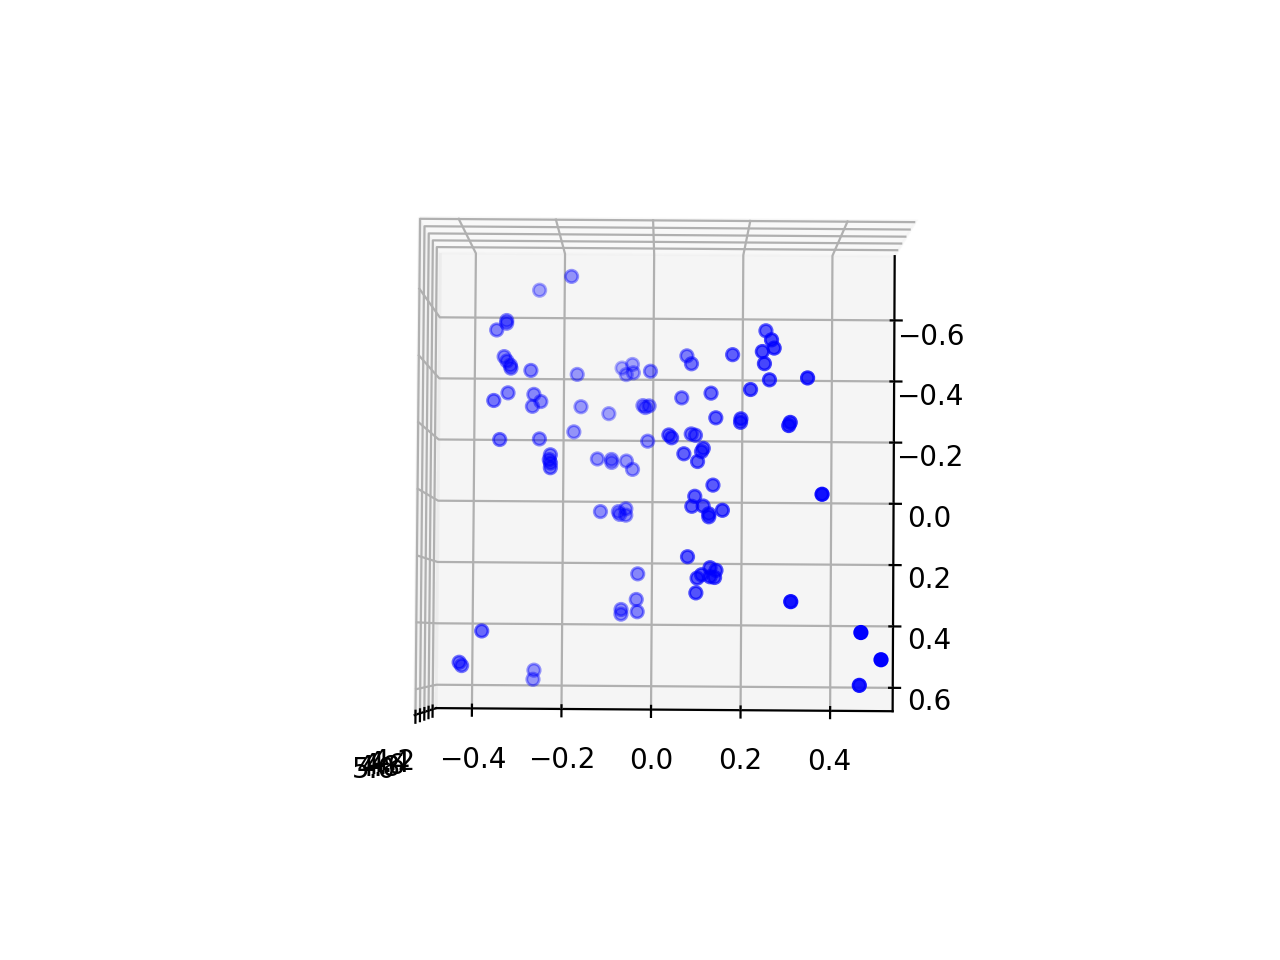
\includegraphics[width=.32\textwidth]{CV/fig/hw5/q353_3_original.png}}
    \subfigure{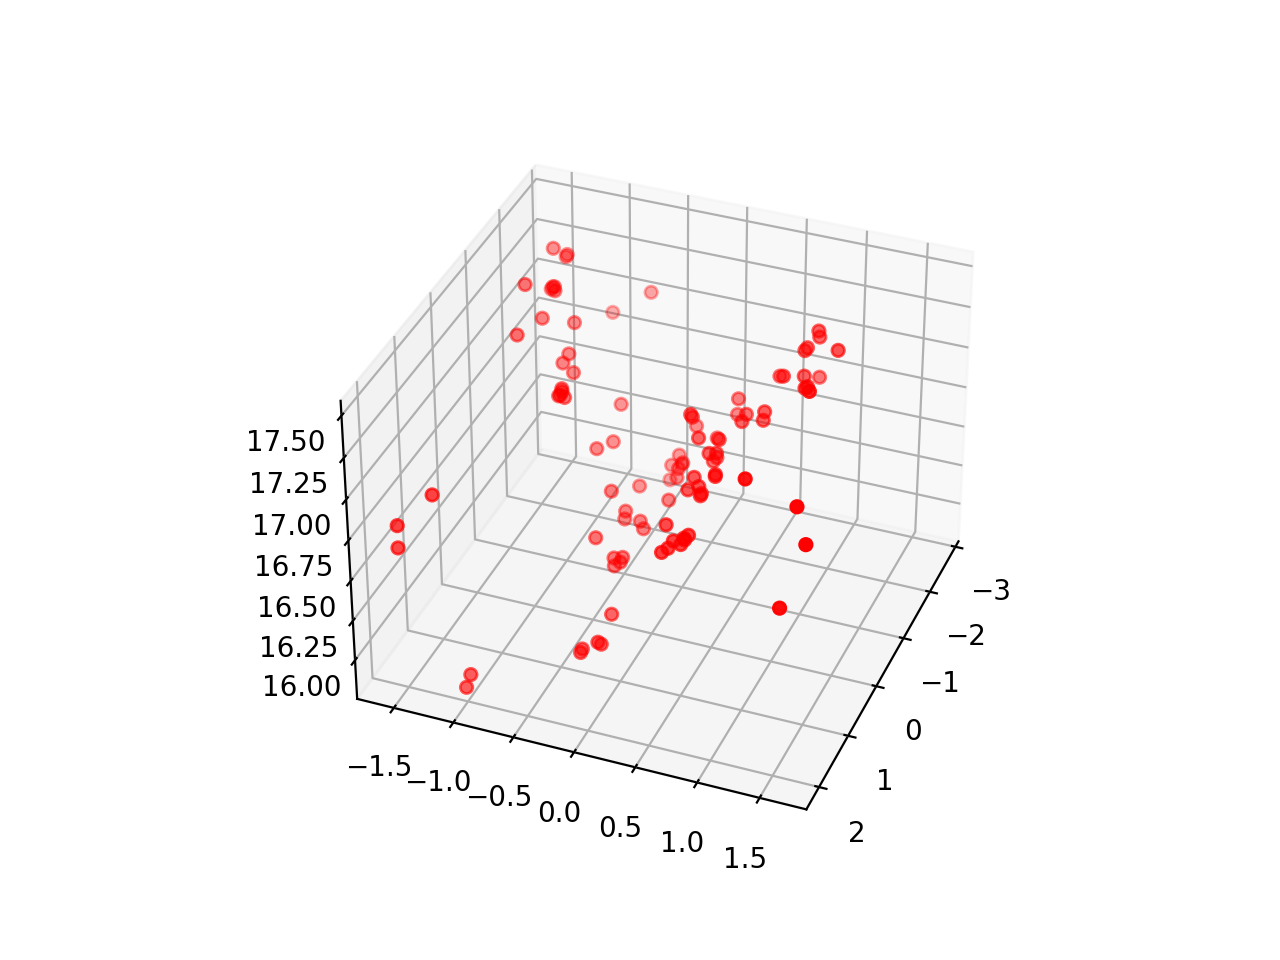
\includegraphics[width=.32\textwidth]{CV/fig/hw5/q353_1.png}}
    \subfigure{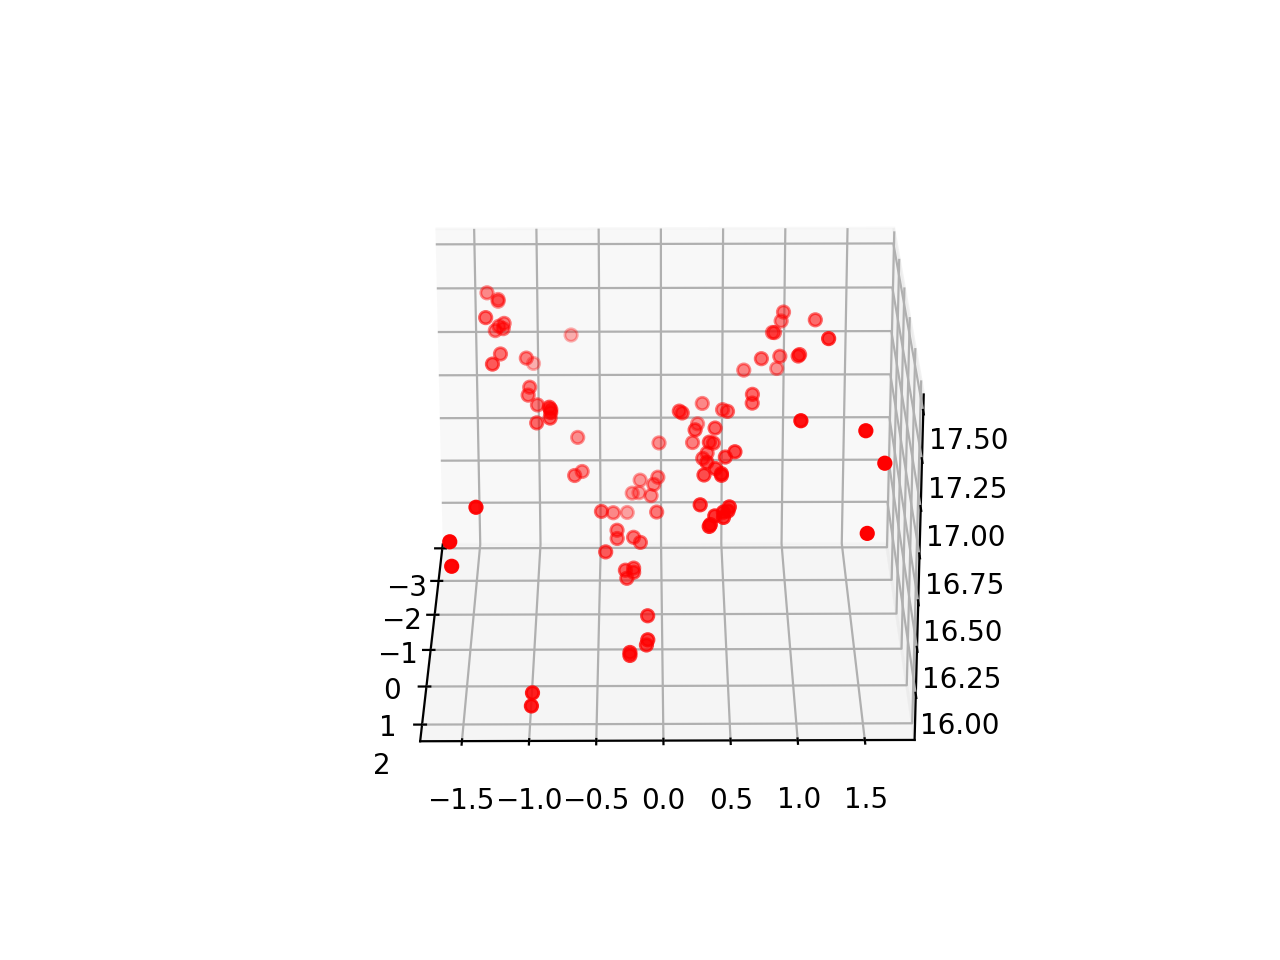
\includegraphics[width=.32\textwidth]{CV/fig/hw5/q353_2.png}}
    \subfigure{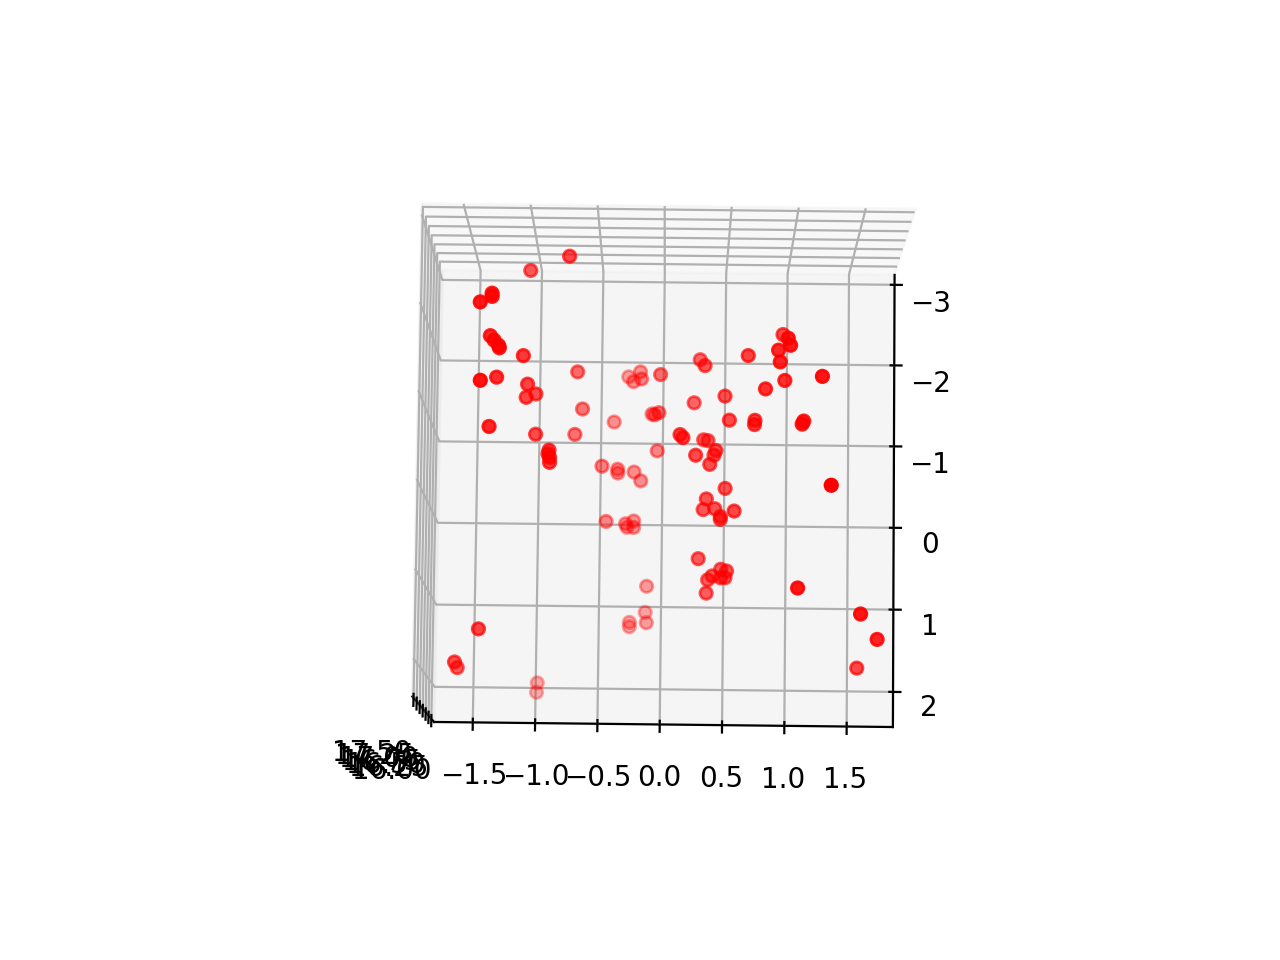
\includegraphics[width=.32\textwidth]{CV/fig/hw5/q353_3.png}}
    \caption{Q3.5.3: Point cloud. Top row: Initial; Bottom row: Optimized.}
    \label{fig:cv_hw5_q353}
\end{figure}

\section{Practice: Calibrated Photometric Stereo}
\subsection{Lambertian Sphere Rendering}

\noindent\textbf{Q4.1} Fig.\ref{fig:cv_hw5_q41} is the result.

\begin{figure}
    \centering
    \subfigure{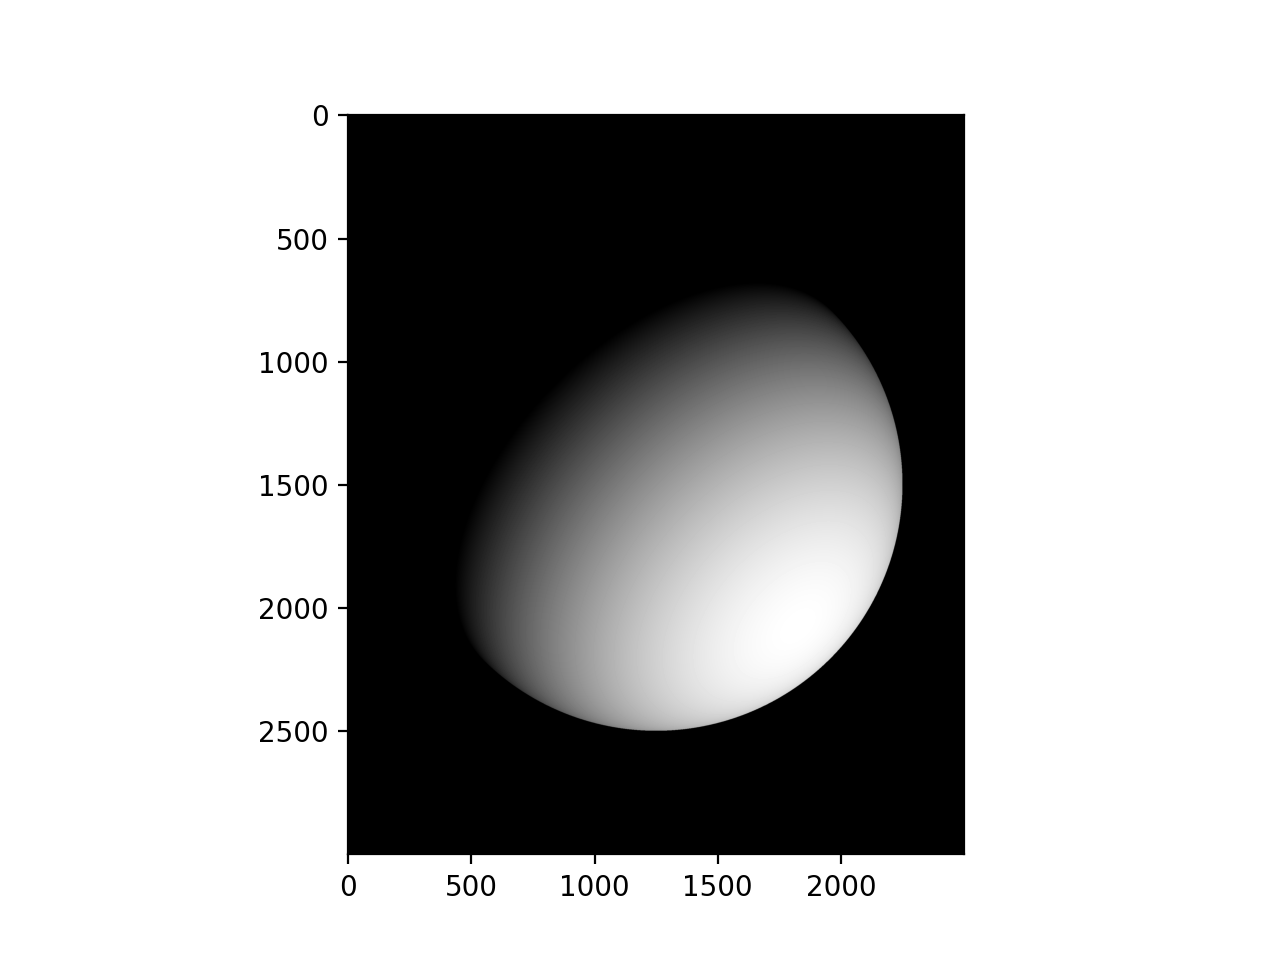
\includegraphics[width=.32\textwidth]{CV/fig/hw5/q41_1.png}}
    \subfigure{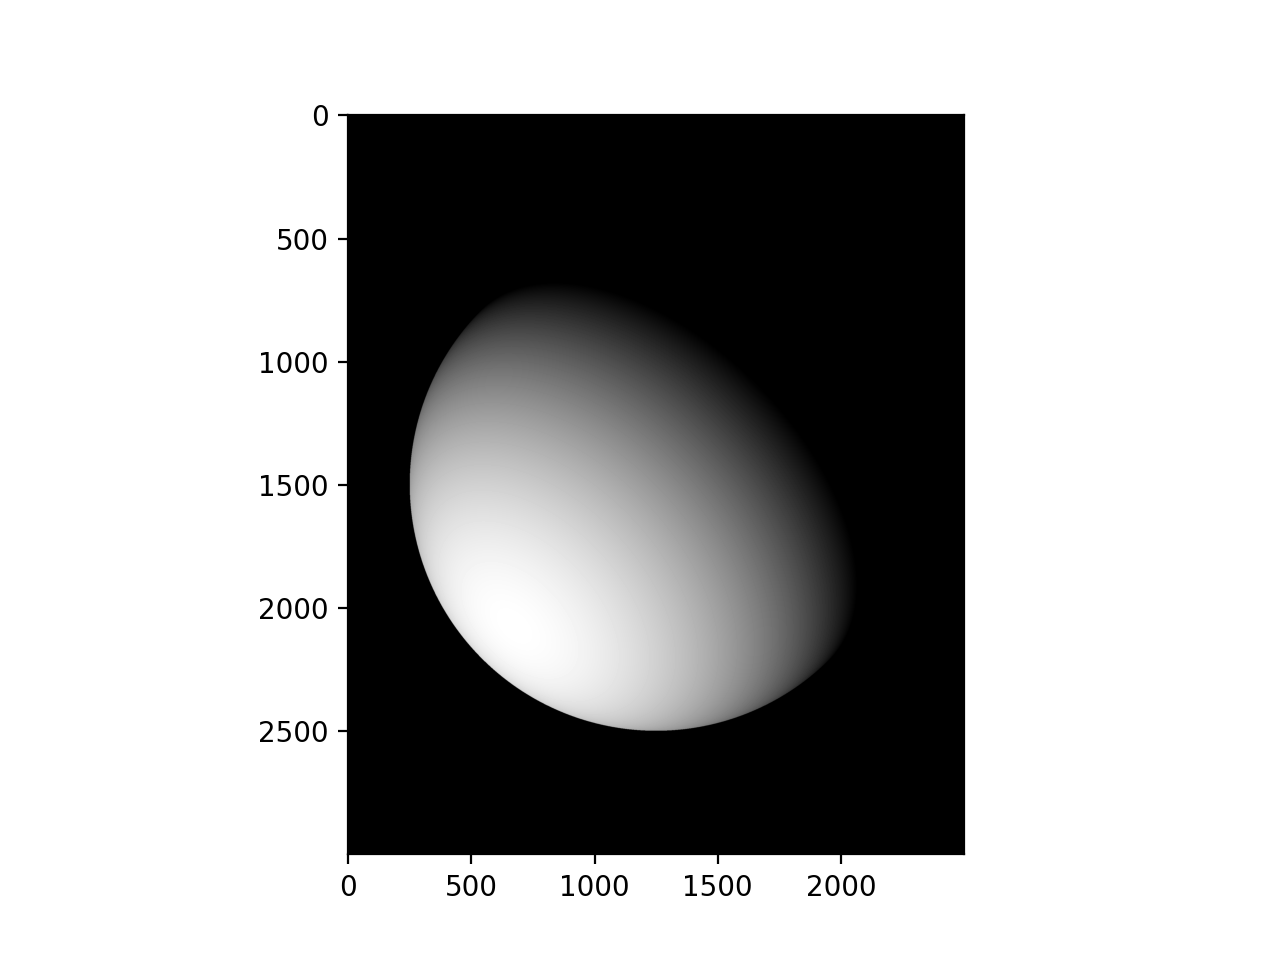
\includegraphics[width=.32\textwidth]{CV/fig/hw5/q41_2.png}}
    \subfigure{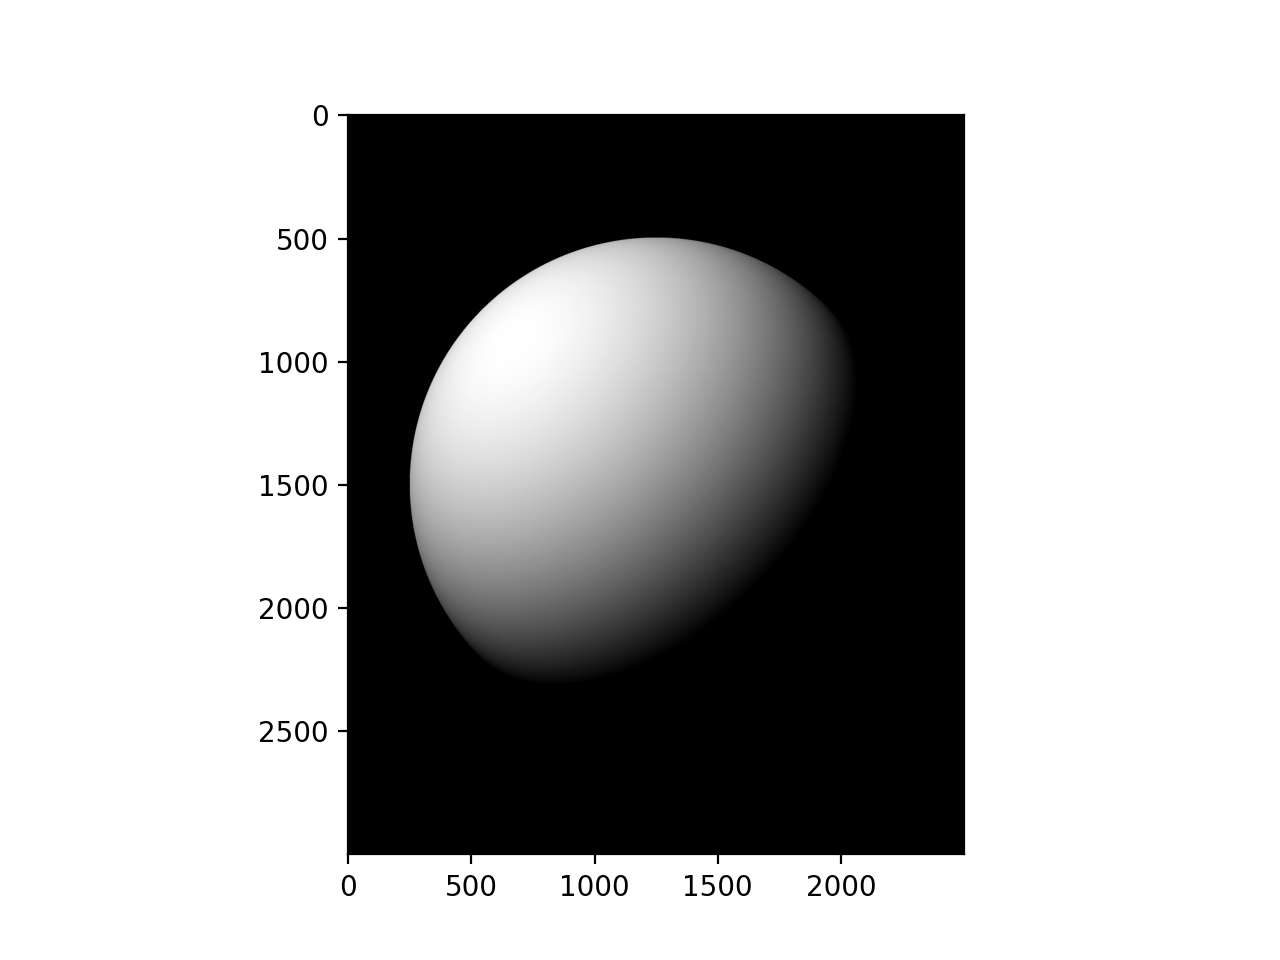
\includegraphics[width=.32\textwidth]{CV/fig/hw5/q41_3.png}}
    \caption{Q4.1: Rendering $n$-dot-$l$ lighting}
    \label{fig:cv_hw5_q41}
\end{figure}

\subsection{Estimating pseudonormals and albedos}
\noindent\textbf{Q4.2.1} See the code for implementation.

\noindent\textbf{Q4.2.2} I regard $A$ as $L^T$ and $y$ as $I$, and use pseudo-inverse to solve the system:

\begin{equation*}
    B = (LL^T)^{-1}LI.
\end{equation*}

\noindent\textbf{Q4.2.3} Fig. \ref{fig:cv_hw5_q423} is the result. The unusual thing about the result is that there are a few high values in the region where shadow appear in the original images, such as ears and necks. One possible reason for this might be, in some training images, those regions are completely in darkness. So it's more difficult to model such regions with less data.

\begin{figure}
    \centering
    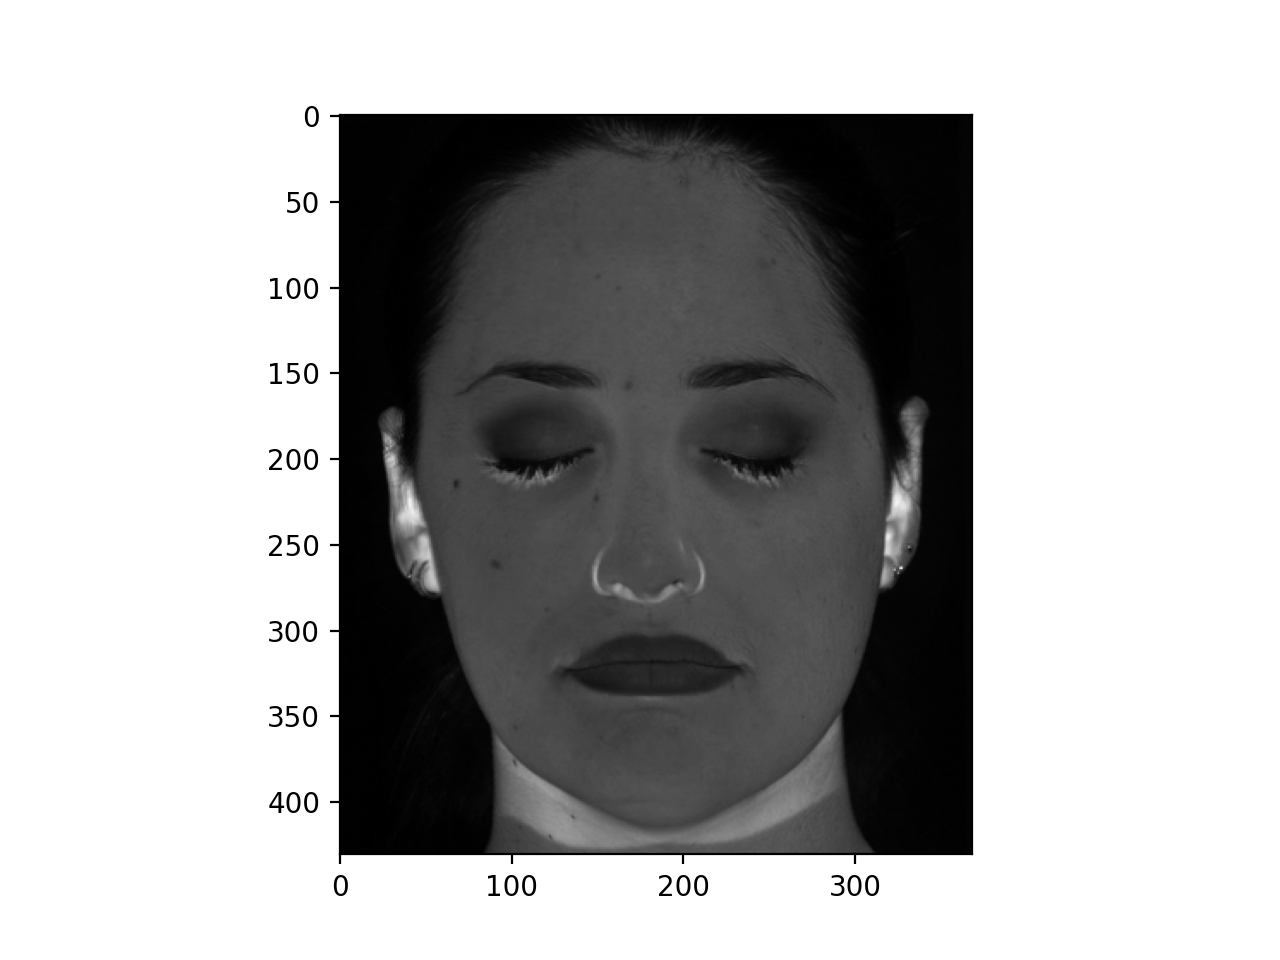
\includegraphics[width=.9\textwidth]{CV/fig/hw5/q423.png}
    \caption{Q4.2.3: Albedos}
    \label{fig:cv_hw5_q423}
\end{figure}

\noindent\textbf{Q4.2.4} Fig. \ref{fig:cv_hw5_q424} is the result. The result matches my expectation of the curvature of the face. From it, we can see a nearly symmetric face shape. 

\begin{figure}
    \centering
    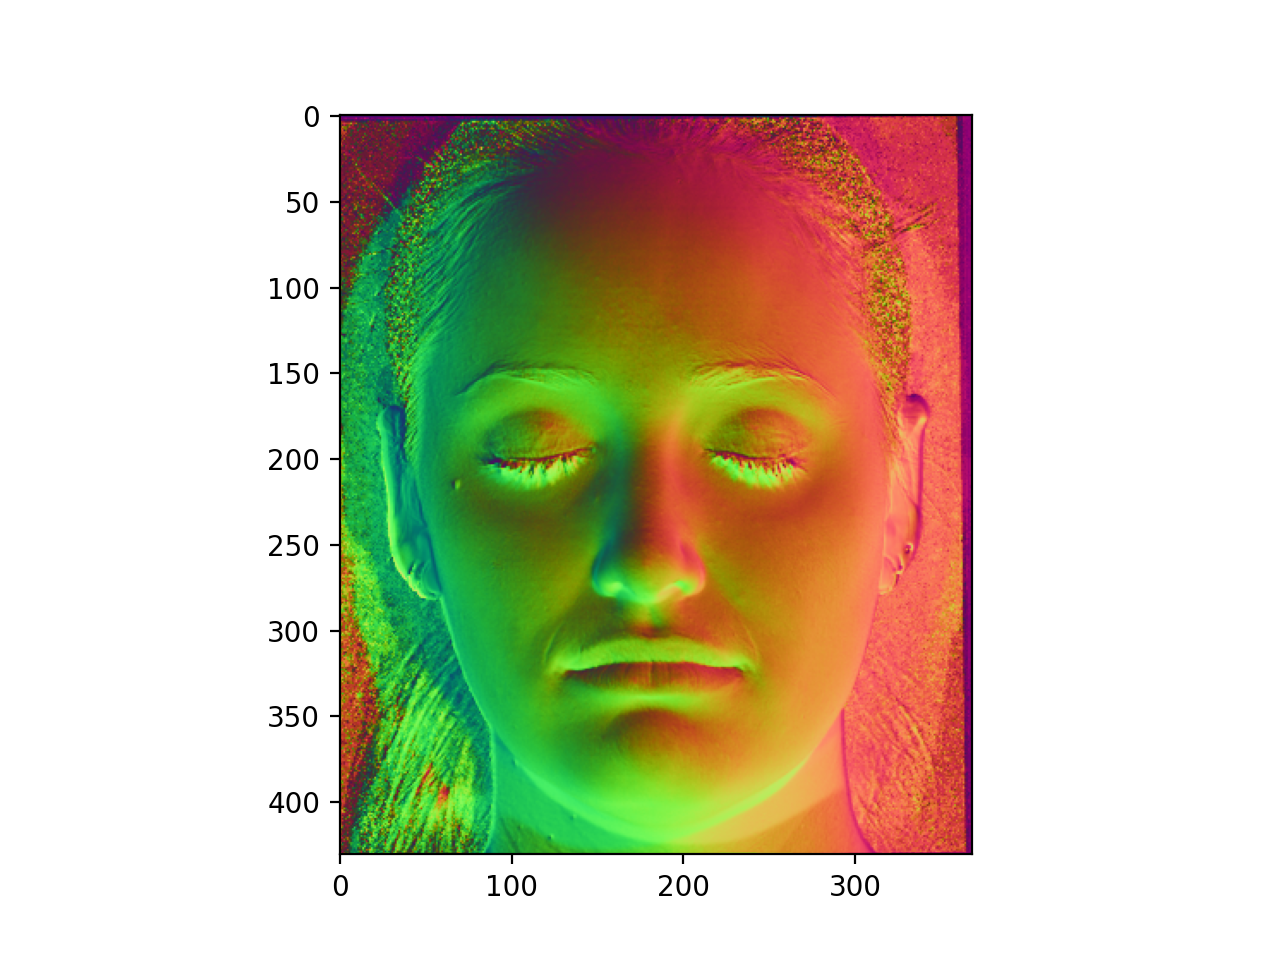
\includegraphics[width=.9\textwidth]{CV/fig/hw5/q424.png}
    \caption{Q4.2.4: Normals}
    \label{fig:cv_hw5_q424}
\end{figure}

\subsection{Depth recovering from normals}

\noindent\textbf{Q4.3.1} Fig.\ref{fig:cv_hw5_q431} is the result. The steps in $integrateFrankot$ can be summarized as:

\begin{itemize}
    \item Calculate FFT of the derivatives of the depth along x and y respectively.
    \begin{equation*}
        P(u,v) = FFT(Z_x(x,y)), Q(u,v) = FFT(Z_y(x,y)).
    \end{equation*}
    \item Calculate FFT $Z_F(u,v)$ of the depth function $Z(x,y)$:
    \begin{equation*}
        Z_F(u, v) = \frac{-juP(u,v)-jvQ(u,v)}{u^2+v^2}.
    \end{equation*}
    \item Calculate $Z(x,y)$ from $Z_F(u,v)$ by iFFT:
    \begin{equation*}
        Z(x,y) = Reg[iFFT(Z_F(u, v))].
    \end{equation*}
    where $Reg[]$ means taking the real part.
\end{itemize}

\begin{figure}
    \centering
    \subfigure{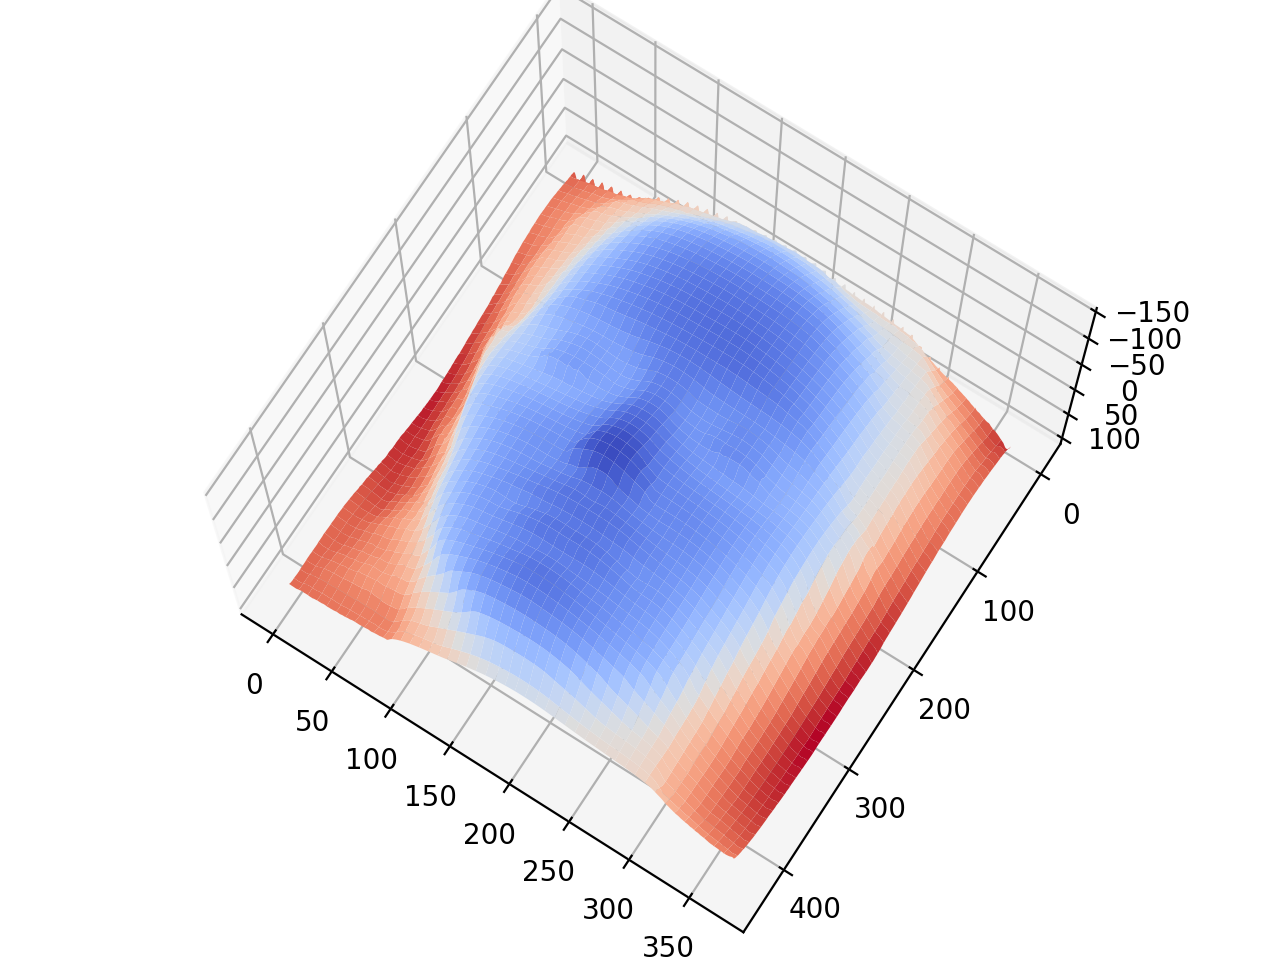
\includegraphics[width=.32\textwidth]{CV/fig/hw5/q431.png}}
    \subfigure{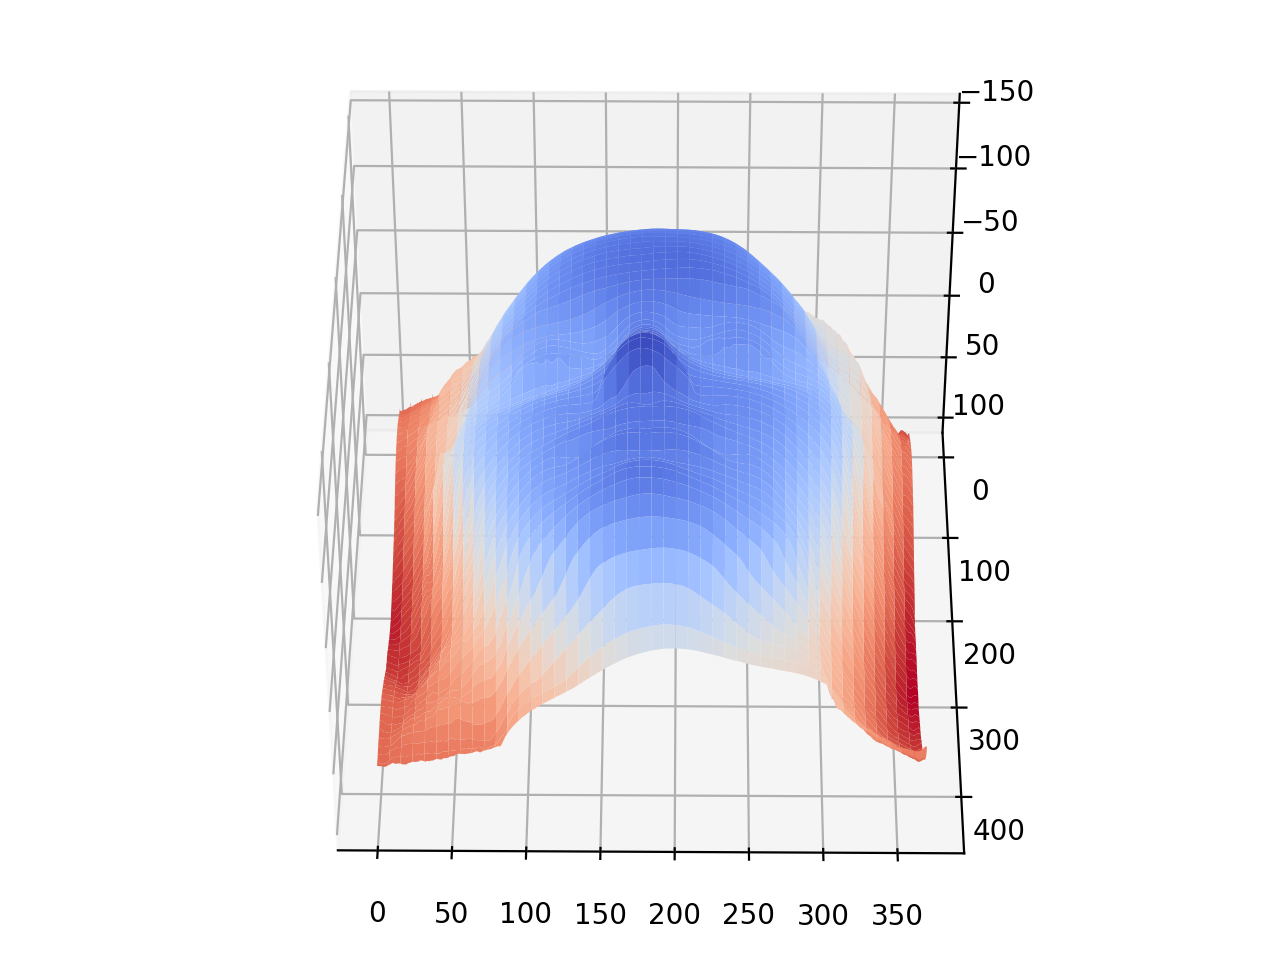
\includegraphics[width=.32\textwidth]{CV/fig/hw5/q431_2.png}}
    \subfigure{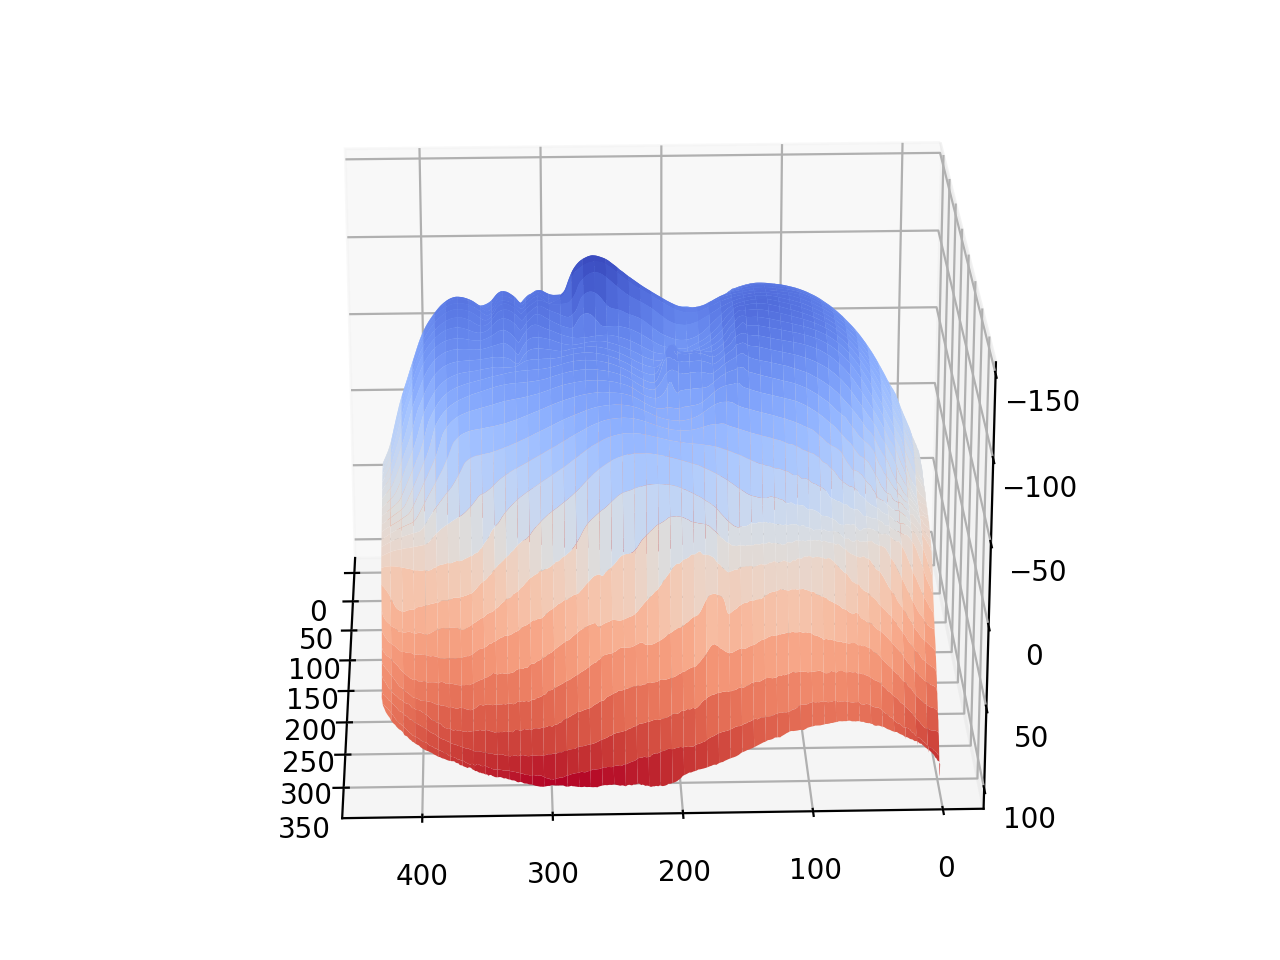
\includegraphics[width=.32\textwidth]{CV/fig/hw5/q431_3.png}}
    \caption{Q4.3.1: Surface}
    \label{fig:cv_hw5_q431}
\end{figure}

\noindent\textbf{Q4.3.2} 
\begin{equation*}
    F(0,0) = \frac{1}{H\cdot W} \sum\limits_{x=0}^{W-1} \sum\limits_{y=0}^{H-1} f(x,y)
\end{equation*}
where $H$ and $W$ is the size of the image.

\end{document}
